
\chapter{Fault-Tolerant Fixed-Time Control of a Twin-Rotor UAV System via Adaptive Neural Networks}
\label{chp3}


\section{Introduction}

In recent years, the use of Unmanned Aerial Vehicles (UAVs) has significantly increased across different domains due to their growing importance in civilian and military applications \cite{UAV_rev, UAV_rev1, Valavanis2015}. Consequently, researchers and industrial companies have put more interest and effort into developing these systems. This ongoing research broadly focuses on improving materials, aerodynamics, electrical components, and control strategies. The primary goal of these advancements is to ensure precise flight, smooth hovering and most importantly safe operation in the presence of expected system failures \cite{Steinberg2021, Zhang2008}. Among the various available platforms, one of the most commonly used flight vehicles is the UAV with two perpendicular rotors, similar to a traditional helicopter \cite{trms_review1, Rahideh2008}. These twin-rotor architectures are highly valued for their agility and Vertical Take-Off and Landing (VTOL) capabilities, making them indispensable for executing complex operations in constrained environments \cite{trms1}.

The precise control of twin-rotor systems presents huge engineering challenges. These vehicles are fundamentally characterized by highly complex, inherently nonlinear dynamics and exhibit strong aerodynamic cross-coupling between their rotational degrees of freedom \cite{NonlinearCoupledDynamics1, trms2}. Furthermore, during real-world flight operations, they are continuously subjected to unpredictable external disturbances and parametric uncertainties arising from varying payloads, aerodynamic ground effects, or shifting environmental conditions \cite{ExternalDisturbances1, ExternalDisturbances2}. Most critically, the operational safety and reliability of these platforms are severely affected by the occurrence of physical faults, such as the partial or total failure of embedded actuators and sensors \cite{Isermann2011, ftc_UAV_review2}. Even minor hardware malfunctions can induce significant trajectory deviations, and ultimately lead to catastrophic system instability if not mitigated promptly and effectively \cite{Steinberg2021, Zhang2008}.

To tackle these profound complexities, a variety of control strategies has been proposed and evaluated in the existing literature. Classical control techniques, such as PID controllers, LQR and $H_{\infty}$ \cite{trmspid, trmsHinf}, alongside conventional nonlinear methods like backstepping, feedback linearization and sliding mode control \cite{trms_smc,trms_bsc, trmsFeedbackL}, have been extensively employed. However, these traditional approaches fundamentally rely on the availability of precise mathematical models and inherently struggle to maintain acceptable performance in the face of severe uncertainties and unmodeled dynamics \cite{control_methods}. To address these limitations, recent advancements have increasingly integrated intelligent approximators, such as Fuzzy Logic Systems and Artificial Neural Networks, to estimate and compensate for unknown nonlinearities online \cite{trmsFuzzyFault, rbfnn2, NN_Control_Ref}. 

Concurrently, various Fault-Tolerant Control (FTC) strategies have been developed to explicitly accommodate hardware failures. Within the literature, these methodologies are fundamentally classified into passive and active paradigms. While  Passive Fault-Tolerant Control (PFTC) approaches utilize fixed, robust control laws designed to render the system inherently insensitive to a predefined set of anticipated faults, Active Fault-Tolerant Control (AFTC) architectures dynamically reconfigure the control structure or parameters in real-time following a failure, by relying on a dedicated Fault Detection and Diagnosis (FDD) mechanism or online estimators to actively identify the fault's magnitude and location. \cite{ftc1, Zhang2013f, fault}. 

Despite these significant strides, a critical gap persists within the current state-of-the-art: in the event of an abrupt and severe fault, traditional asymptotic or even finite-time controllers may not react with sufficient rapidity, as their convergence times remain intrinsically linked to the system's initial states \cite{Bhat2000, Polyakov2012}. In safety-critical aerospace applications, there is an indispensable need for fast fault compensation and rigorous state convergence within a strict, pre-calculated short period that is completely independent of the initial conditions \cite{fxt, Zuo2018}. In\cite{panda2025} they proposed a fault-tolerant sliding mode controller (FT-SMC) combined with a sliding-mode observer (FT-SMO) for the TRMS, designed to manage parametric uncertainties, exogenous disturbances, and sensor/actuator imperfections simultaneously. While this work demonstrates commendable robustness on the same benchmark platform, the inherent use of a discontinuous sliding mode law introduces control chattering, which can degrade actuator longevity. Moreover, it provides only asymptotic convergence guarantees without bounding the settling time independently of initial conditions, a critical limitation in safety-sensitive aerial missions. In a related direction, \cite{zhang2025_rbf} developed a passive fault-tolerant controller combining sliding mode control with radial basis function (RBF) neural networks for UAVs, where an enhanced PSO-based optimization tunes the network parameters to alleviate chattering. However, the passive nature of this scheme implies no explicit online estimation or compensation of the fault signal itself, which limits its adaptability to unforeseen fault types. Furthermore, this approach provides no fixed-time convergence guarantee.

To overcome this critical limitation, this chapter develops a novel Fixed-Time Fault-Tolerant Adaptive Neural Network Controller \cite{my1article, Bacha2024}. The proposed control strategy is based on the backstepping technique, mathematically augmented and formulated to guarantee fixed-time stability \cite{lemma2}. To dynamically compensate for the unknown nonlinearities, external aerodynamic disturbances, and sudden fault occurrences, mainly in sensors, Radial Basis Function Neural Networks (RBFNN) are effectively integrated into the control loop to provide accurate online estimations of lumped uncertainties \cite{Park1991, rbfnn1}. Furthermore, to overcome the persistent and computational challenge of manual, trial-and-error parameter tuning, a metaheuristic optimization algorithm specifically, the Grey Wolf Optimizer (GWO) is utilized \cite{gwo}. The GWO systematically navigates the parameter search space to optimally tune the controller gains, ensuring a delicate and vital balance between high-precision tracking accuracy and the generation of smooth control efforts \cite{9064786, glida_thesis}.

To rigorously validate the theoretical efficacy of the proposed control architecture, the Twin Rotor Multiple Input Multiple Output System (TRMS) is adopted as the primary benchmark experimental platform.  The TRMS is a highly nonlinear, grounded aerodynamic prototype whose dynamic behavior closely mimics that of a complex helicopter, particularly exhibiting pronounced cross-coupling between its main and tail rotors \cite{Juang2005, trms4}. This significant dynamical complexity makes the TRMS an exceptionally challenging and ideal testbed for developing, evaluating, and refining advanced fault-tolerant control strategies prior to their deployment on unconstrained free-flying UAVs \cite{trms3}.

The primary contributions of this chapter are consequently multifaceted and address both theoretical and practical dimensions of UAV control. Primarily, this work establishes a robust control framework that ensures the fixed-time stability and precise trajectory tracking of the aerial system despite the simultaneous presence of severe sensor faults, and environmental disturbances. Additionally, the integration of the GWO algorithm effectively eliminates the subjectivity and inefficiency associated with manual controller tuning. The fundamental methodologies and core findings detailed in this chapter form the basis of our work published in the journal \textit{Drones} \cite{my1article}.

%The remainder of this chapter is organized as follows. Section \ref{sec:trms_modeling} provides a detailed mathematical formulation of the TRMS, explicitly incorporating the nonlinear dynamic equations alongside the modeled sensor faults. Following this, the core control design procedure and the rigorous fixed-time stability analysis using Lyapunov theory are presented in Section \ref{sec:trms_control_design}. The metaheuristic optimization process utilizing the GWO is then detailed in Section \ref{sec:trms_optimization}, highlighting the formulation of the multi-objective cost function. Finally, comprehensive numerical simulation results are presented and discussed in Section \ref{sec:trms_results} to demonstrate the superiority and robustness of the proposed approach, before concluding the chapter with a summary of the key findings in Section \ref{sec:trms_conclusion}.
\section{Dynamic Model and System Representation}
\label{sec:trms_modeling}

The TRMS is a laboratory apparatus designed to emulate the complex flight dynamics of a helicopter, making it a suitable benchmark for testing advanced control strategies \cite{trms1,trms2,trms3}. It features two rotors: a main rotor that influences the pitch motion and a tail rotor that affects the yaw motion \cite{trms4}. These rotors are mounted on a beam, which is pivoted to allow for pitch and yaw movements around its central axis. The control of these motions is achieved by adjusting the input voltages to the electric motors driving each rotor. The inherent characteristics of the TRMS, such as strong coupling between pitch and yaw dynamics, nonlinearities, and susceptibility to uncertainties and disturbances, present significant control challenges.

\begin{figure}
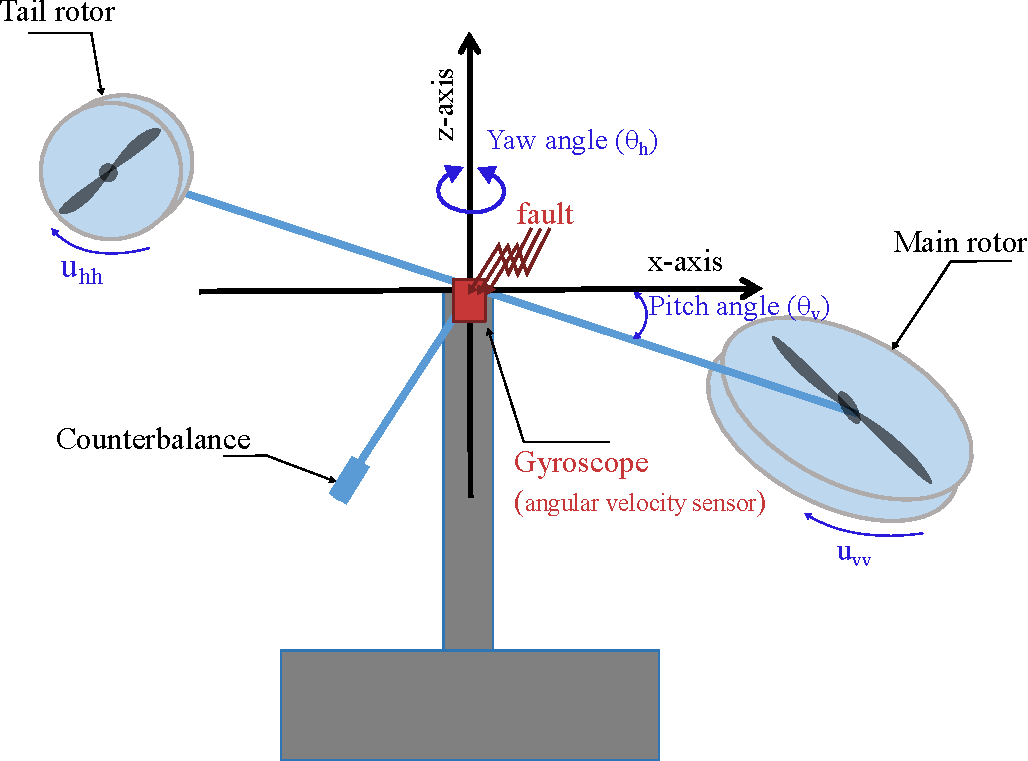
\includegraphics[width=10cm]{figure3/trms.pdf}
\caption{Structural and functional layout of the TRMS. \label{trms}}
\end{figure}

\subsection{Nonlinear Dynamic Model}
The complete nonlinear model describing the flight dynamics of the TRMS in both the vertical (pitch) and horizontal (yaw) planes is derived from fundamental physics principles. Let $\alpha_P$ and $\alpha_Y$ denote the pitch and yaw angles, respectively. Their corresponding angular velocities are $\omega_P = \dot{\alpha}_P$ and $\omega_Y = \dot{\alpha}_Y$. The dynamics are given by a set of coupled differential equations.

The pitch motion dynamics can be described as:
\begin{equation}
    \label{eq:pitch_dyn_full}
    \begin{cases}
        \dot{\alpha}_P = \omega_P \\
        \begin{aligned}
            J_P \dot{\omega}_P &= (\kappa_{P,1} M_{P}^2 + \kappa_{P,2} M_{P})(1 - K_{cpl} \omega_Y \cos(\alpha_P)) - M_g \sin(\alpha_P) \\
            &\quad - B_P \omega_P + K_{gyr} \omega_Y^2 \sin(2\alpha_P) + \tau_{dP}(t)
        \end{aligned} \\
        T_{P,1} \dot{M}_{P} = -T_{P,0} M_{P} + k_P v_P
    \end{cases}
\end{equation}
and the yaw motion dynamics as:
\begin{equation}
    \label{eq:yaw_dyn_full}
    \begin{cases}
        \dot{\alpha}_Y = \omega_Y \\
        J_Y \dot{\omega}_Y = \kappa_{Y,1} M_{Y}^2 + \kappa_{Y,2} M_{Y} - B_Y \omega_Y - M_{cr} + \tau_{dY}(t) \\
        T_{Y,1} \dot{M}_{Y} = -T_{Y,0} M_{Y} + k_Y v_Y
    \end{cases}
\end{equation}
where $J_P$ and $J_Y$ are the moments of inertia for the pitch and yaw axes, respectively. The terms $M_{P}$ and $M_{Y}$ represent the momentums generated by the main and tail DC motors, which are assumed to be measurable. The control input voltages applied to the main and tail motors are denoted by $v_P$ and $v_Y$, respectively. The aerodynamic coefficients for the main and tail rotors are $\kappa_{P,1}, \kappa_{P,2}, \kappa_{Y,1},$ and $\kappa_{Y,2}$. $K_{cpl}$ represents a coupling factor accounting for the influence of yaw velocity on pitch dynamics, while $M_g$ is the gravitational torque component affecting the pitch motion. The friction coefficients for pitch and yaw movements are $B_P$ and $B_Y$, and $K_{gyr}$ is a gyroscopic effect coefficient. The time constants and gains for the main motor dynamics are $T_{P,1}, T_{P,0},$ and $k_P$, and for the tail motor dynamics, they are $T_{Y,1}, T_{Y,0},$ and $k_Y$. Lastly, $\tau_{dP}(t)$ and $\tau_{dY}(t)$ are external disturbances affecting the pitch and yaw motions, respectively, which are assumed to be bounded with unknown upper limits.
The term $M_{cr}$ in Eq. \eqref{eq:yaw_dyn_full} represents the cross-reaction momentum from the main rotor affecting the yaw dynamics. It can be expressed in the time domain as:
\begin{equation}
    \label{eq:cross_reaction}
    M_{cr}(t) = c_{cr} k_{c} e^{-\lambda t} (\kappa_{P,1} M_{P}^2 + \kappa_{P,2} M_{P})
\end{equation}
where $c_{cr}$, $k_{c}$, and $\lambda$ are constants related to this cross-coupling effect. The detailed parameters and their numerical values are typically provided by the system manufacturer or can be identified experimentally. The model presented in Eqs. \eqref{eq:pitch_dyn_full} and \eqref{eq:yaw_dyn_full} is primarily used for simulation purposes, while the controller design often benefits from a simplified representation.

\subsection{Decoupled System Representation}
For control design simplification, the TRMS model can be decoupled into two subsystems representing the pitch (vertical) and yaw (horizontal) motions independently. This approach treats the complex interactions and gyroscopic effects as part of lumped disturbances acting on each subsystem.

The decoupled model for the pitch subsystem is:
\begin{equation}
    \label{eq:pitch_decoupled}
    \begin{cases}
        \dot{\alpha}_P = \omega_P \\
        J_P \dot{\omega}_P = \kappa_{P,1} M_{P}^2 + \kappa_{P,2} M_{P} - M_g \sin(\alpha_P) - B_P \omega_P + \Delta_P \\
        T_{P,1} \dot{M}_{P} = -T_{P,0} M_{P} + k_P v_P
    \end{cases}
\end{equation}
with $\Delta_P = -(\kappa_{P,1} M_{P}^2 + \kappa_{P,2} M_{P}) K_{cpl} \omega_Y \cos(\alpha_P) + K_{gyr} \omega_Y^2 \sin(2\alpha_P) + \tau_{dP}(t)$, for the yaw subsystem:
\begin{equation}
    \label{eq:yaw_decoupled}
    \begin{cases}
        \dot{\alpha}_Y = \omega_Y \\
        J_Y \dot{\omega}_Y = \kappa_{Y,1} M_{Y}^2 + \kappa_{Y,2} M_{Y} - B_Y \omega_Y + \Delta_Y \\
        T_{Y,1} \dot{M}_{Y} = -T_{Y,0} M_{Y} + k_Y v_Y
    \end{cases}
\end{equation}
where $\Delta_Y = -M_{cr} + \tau_{dY}(t)$.   $\Delta_P$ and $\Delta_Y$ are the lumped uncertainties and disturbances for the pitch and yaw subsystems, respectively, grouping cross-coupling effects, gyroscopic moments, and external disturbances.

\subsection{System Model with Sensor Faults}
To investigate fault-tolerant control, we consider faults affecting the angular velocity sensors (gyroscopes). Let the state vectors for the pitch and yaw subsystems be defined as $\chi_P = [\chi_{P,1}, \chi_{P,2}, \chi_{P,3}]^T = [\alpha_P, \omega_P, M_{P}]^T$ and $\chi_Y = [\chi_{Y,1}, \chi_{Y,2}, \chi_{Y,3}]^T = [\alpha_Y, \omega_Y, M_{Y}]^T$. It is assumed that these state variables are measurable.

The measured outputs from the sensors, denoted by $y_i = [y_{i,1}, y_{i,2}, y_{i,3}]^T$ for $i \in \{P, Y\}$, can be affected by faults as follows:
\begin{equation}
    \label{eq:sensor_fault_model}
    \begin{cases}
        y_{i,1} = \chi_{i,1} \\
        y_{i,2} = g_{M,i} \chi_{i,2}(t) + g_{A,i}(t) \\
        y_{i,3} = \chi_{i,3}
    \end{cases}
\end{equation}
The measurement $y_{i,1}$ (angle) and $y_{i,3}$ (motor momentum) are assumed to be fault-free, while the angular velocity measurement $y_{i,2}$ is subject to faults. The term $g_{A,i}(t)$ represents additive faults such as bias, drift, or loss of accuracy, while $g_{M,i}(t)$ represents multiplicative faults, primarily modeling a sensor's loss of effectiveness.
Only the potentially faulty measurements $y_i$ are available to the controller. The types of sensor faults considered are:
\begin{itemize}
    \item \textbf{Bias}: A constant offset added to the true sensor output.
    $y_{i,2}(t) = \chi_{i,2}(t) + g_{A,i}$, where $g_{A,i}$ is a non-zero constant after fault occurrence time $t_{\text{fault}}$, and $\dot{g}_{A,i} = 0$.
    \item \textbf{Drift}: A slow, typically linear, time-varying offset added to the sensor output.
    $y_{i,2}(t) = \chi_{i,2}(t) + g_{A,i}(t)$, where $|g_{A,i}(t)| = \delta_i t$ with $0 < \delta_i \ll 1$ for $t \ge t_{\text{fault}}$.
    \item \textbf{Loss of Accuracy}: Random fluctuations or noise added to the sensor output.
    $y_{i,2}(t) = \chi_{i,2}(t) + g_{A,i}(t)$, where $|g_{A,i}(t)| < g_{A0,i}$ (a bound) and $\dot{g}_{A,i} \neq 0$ for $t \ge t_{\text{fault}}$.
    \item \textbf{Loss of Effectiveness}: A scaling down of the true sensor output.
    $y_{i,2}(t) = g_{M,i}(t) \chi_{i,2}(t)$, where $0 < g_{M0,i} \le g_{M,i}(t) \le 1$ for $t \ge t_{\text{fault}}$.
\end{itemize}
The terms $g_{A,i}(t)$ and $g_{M,i}(t)$ are assumed to be smoothly varying within their respective bounds $[ -g_{A0,i}, g_{A0,i} ]$ and $[ g_{M0,i}, 1 ]$.

The sensor fault model in Eq. \eqref{eq:sensor_fault_model} can be conveniently rewritten by defining an equivalent sensor fault term, $S_{i,eq}(t, \chi_{i,2})$, as:
\begin{equation}
    \label{eq:equivalent_fault}
    y_{i,2}(t) = \chi_{i,2}(t) + S_{i,eq}(t, \chi_{i,2})
\end{equation}
where $S_{i,eq}(t, \chi_{i,2}) = (g_{M,i}(t)-1)\chi_{i,2}(t) + g_{A,i}(t)$ encompasses all the aforementioned fault types.

Using the measured (and potentially faulty) states $y_i$, and substituting $\chi_{i,2} = y_{i,2} - S_{i,eq}$, the state-space representation of the $i$-th subsystem (for $i \in \{P,Y\}$ corresponding to pitch and yaw respectively) suitable for control design becomes:
\begin{equation}
    \label{eq:system_for_control_design}
    \begin{cases}
        \dot{y}_{i,1} = y_{i,2} - S_{i,eq} \\
        \dot{y}_{i,2} = \Psi_{i,1}(\mathbf{y}_i) + y_{i,3} + D_i(t) + \dot{S}_{i,eq} \\
        \dot{y}_{i,3} = \Psi_{i,2}(\mathbf{y}_i) + u_i
    \end{cases}
\end{equation}
where $\Psi_{i,1}(\cdot)$ and $\Psi_{i,2}(\cdot)$ represent unknown nonlinear functions of the TRMS dynamics, $D_i(t)$ incorporates the lumped disturbances and some dynamic terms not directly dependent on $y_{i,3}$ or $u_i$. The functions $\Psi_{i,1}$ and $\Psi_{i,2}$ and the equivalent fault $S_{i,eq}$ (and its derivative) are generally unknown and will be estimated or compensated for by the adaptive fault-tolerant control scheme. The primary control objective is to design $u_i$ such that $y_{i,1}$ tracks a desired reference trajectory $y_{d,i,1}$ despite these uncertainties, disturbances, and sensor faults.

\section{Control Design and Stability Analysis}
\label{sec:trms_control_design}

This section details the design of the Fault-Tolerant Fixed-Time Adaptive Neural Controller (FTFxTANC) for the TRMS. The primary objective is to develop a robust control law that ensures fixed-time tracking of desired reference signals for both pitch and yaw angles, despite unknown nonlinear dynamics, external disturbances, and various types of sensor faults. The control strategy is based on the backstepping technique, enhanced by RBFNNs for online approximation of unknown functions combined with adaptive estimators for fault compensation. The overall control architecture is schematically illustrated in Fig.~\ref{fig:control_architecture}. To achieve the best performance of TRMS motions, the control parameters are tuned using the GWO optimization algorithm.

\begin{figure}
    \centering
    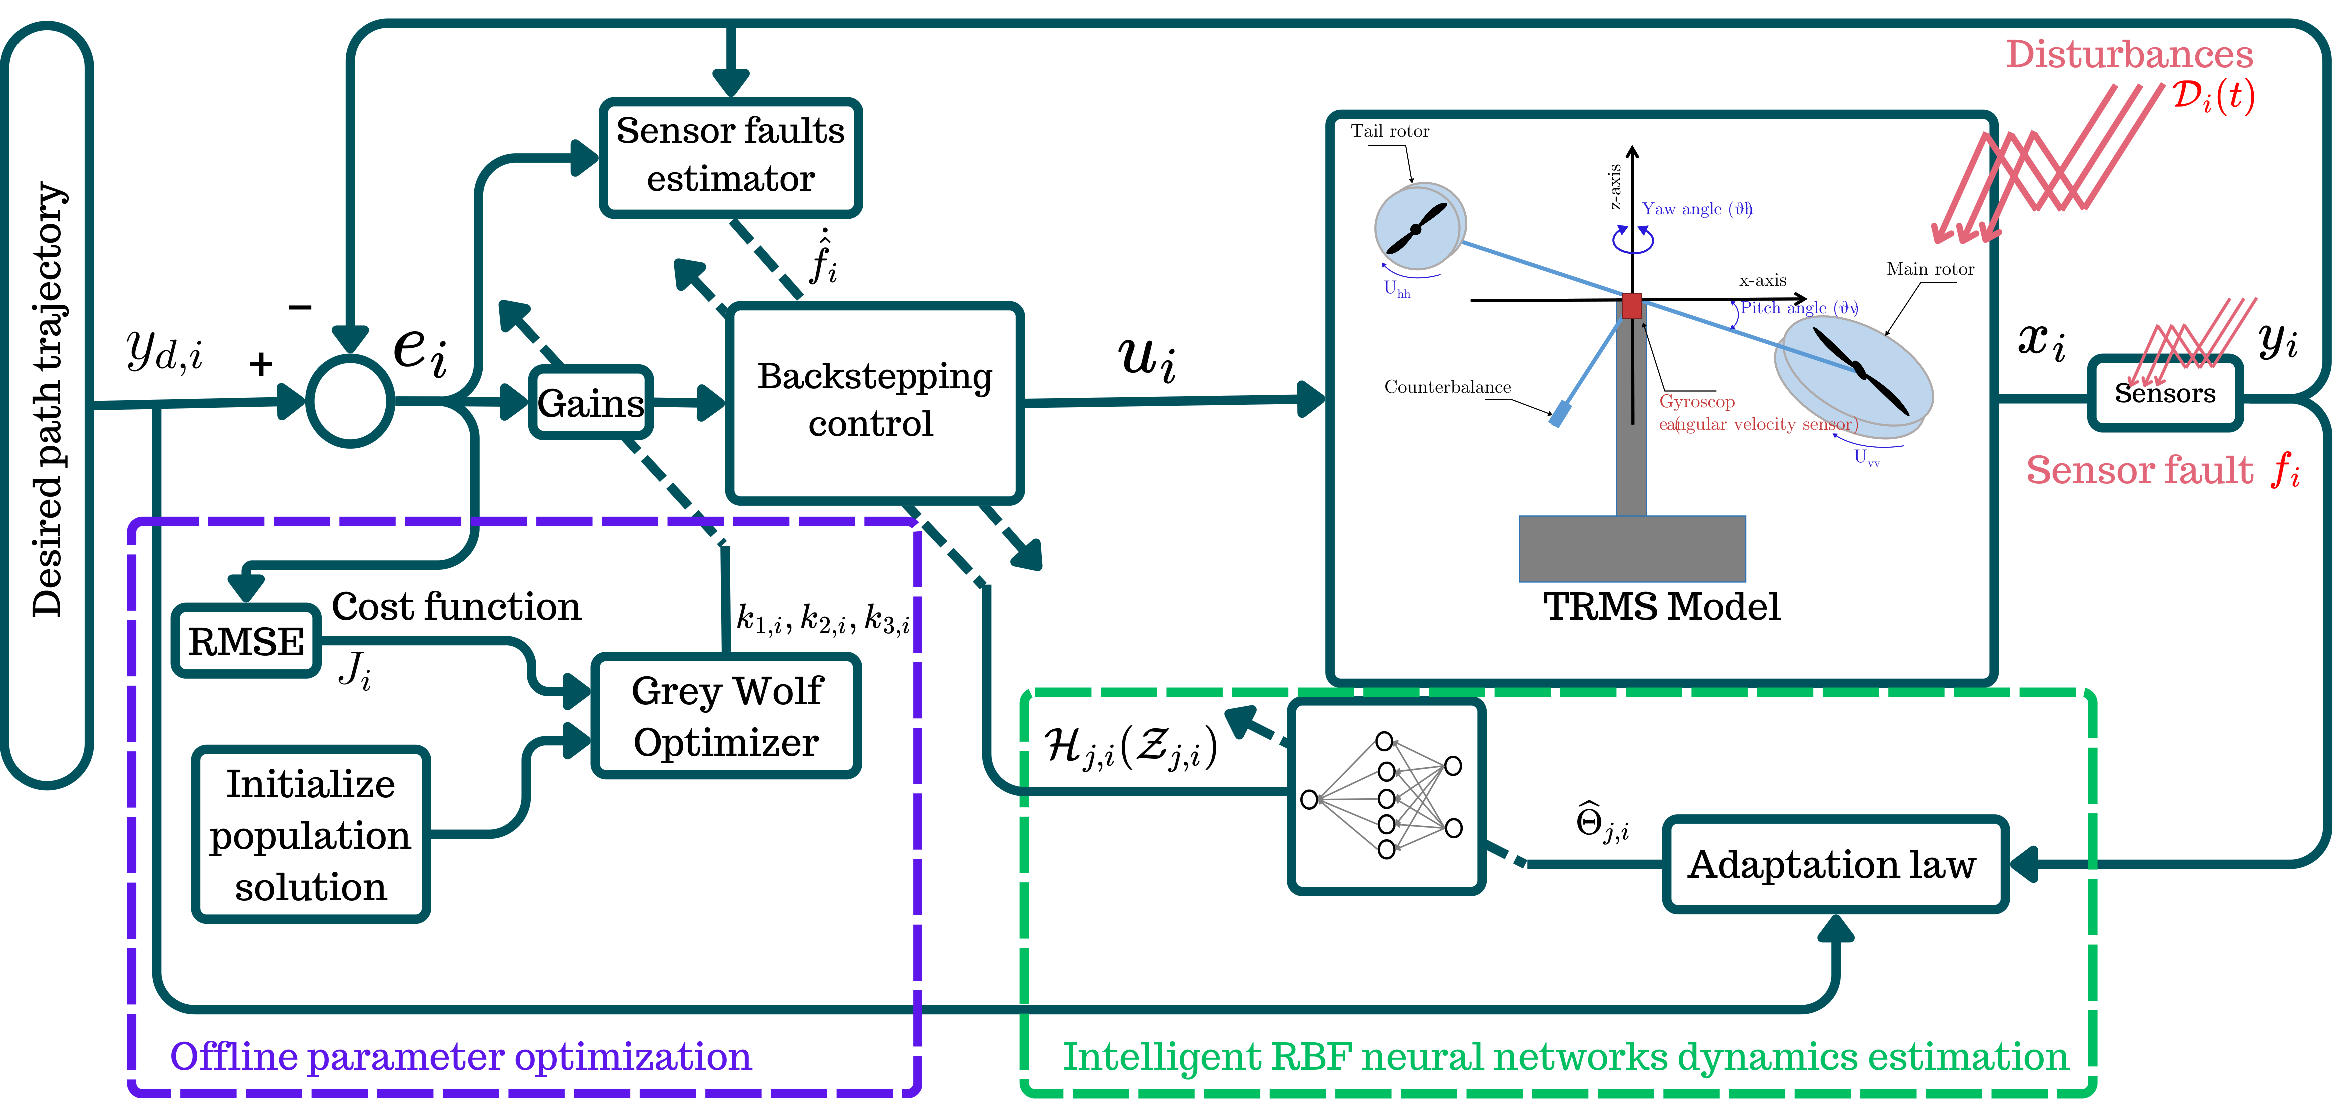
\includegraphics[width=14cm]{figure3/scheme.pdf}
    \caption{Schematic of the proposed fixed-time fault-tolerant adaptive neural control architecture for the TRMS. \label{fig:control_architecture}}
\end{figure}

The design procedure follows a step-by-step backstepping approach for each subsystem $i \in \{P,Y\}$ (pitch and yaw), based on the system representation given by Eq.~(3.9).

\subsection{Step 1: Tracking Error and Virtual Control Design}
We define the tracking errors for each subsystem $i$ as follows:
\begin{align}
    e_{i,1} &= y_{i,1} - y_{d,i} \label{eq:error_e1} \\
    e_{i,2} &= y_{i,2} - \alpha_{i,1} \label{eq:error_e2} \\
    e_{i,3} &= y_{i,3} - \alpha_{i,2} \label{eq:error_e3}
\end{align}
where $y_{d,i}$ is the desired reference trajectory, and $\alpha_{i,1}$ and $\alpha_{i,2}$ are virtual control laws to be designed in subsequent steps.

The derivative of the first error term $e_{i,1}$ is obtained by taking the derivative of Eq.~\eqref{eq:error_e1} and substituting $\dot{y}_{i,1} = y_{i,2} - S_{i,eq}$ from the system dynamics in Eq.~(3.9):
\begin{align}
    \dot{e}_{i,1} &= \dot{y}_{i,1} - \dot{y}_{d,i} \nonumber \\
    &= (y_{i,2} - S_{i,eq}) - \dot{y}_{d,i} \nonumber \\
    &= (e_{i,2} + \alpha_{i,1}) - S_{i,eq} - \dot{y}_{d,i} \label{eq:e1_dot}
\end{align}

Consider the first Lyapunov function candidate for both subsystems:
\begin{equation}
    \mathcal{L}_1 = \sum_{i \in \{P,Y\}} \frac{1}{2} \left( e_{i,1}^2 + \frac{1}{\gamma_{S,i}} \widetilde{S}_{i,eq}^2 \right) \label{eq:lyapunov_L1}
\end{equation}
where $\gamma_{S,i}$ is a positive design constant and $\widetilde{S}_{i,eq} = S_{i,eq} - \widehat{S}_{i,eq}$ is the estimation error of the equivalent sensor fault, with $\widehat{S}_{i,eq}$ being its adaptive estimate.

The time derivative of $\mathcal{L}_1$ is given by:
\begin{align}
    \dot{\mathcal{L}}_1 &= \sum_{i \in \{P,Y\}} \left( e_{i,1} \dot{e}_{i,1} + \frac{1}{\gamma_{S,i}} \widetilde{S}_{i,eq} (\dot{S}_{i,eq} - \dot{\widehat{S}}_{i,eq}) \right) \nonumber \\
    &= \sum_{i \in \{P,Y\}} \left( e_{i,1} (e_{i,2} + \alpha_{i,1} - S_{i,eq} - \dot{y}_{d,i}) + \frac{1}{\gamma_{S,i}} \widetilde{S}_{i,eq} (\dot{S}_{i,eq} - \dot{\widehat{S}}_{i,eq}) \right) \label{eq:L1_dot_expanded}
\end{align}

To ensure fixed-time convergence, the virtual control law $\alpha_{i,1}$ and the adaptive fault estimator $\widehat{S}_{i,eq}$ are designed as:
\begin{align}
    \alpha_{i,1} &\triangleq \dot{y}_{d,i} + \widehat{S}_{i,eq} - c_{i,1} e_{i,1}^{2\rho_1-1} \label{eq:alpha1} \\
    \dot{\widehat{S}}_{i,eq} &\triangleq \gamma_{S,i} (-e_{i,1} + c_{S,i} \widetilde{S}_{i,eq}^{2\rho_1-1} + d_{S,i} \widetilde{S}_{i,eq}^{2\rho_2-1}) \label{eq:f_hat_dot}
\end{align}
where $c_{i,1}$, $c_{S,i}$, and $d_{S,i}$ are positive design parameters, and $\rho_1, \rho_2$ are constants for fixed-time stability (typically $0 < \rho_1 < 1$ and $\rho_2 > 1$, as in Lemma \ref{lemma2} of the paper).
Substituting Eqs.~\eqref{eq:alpha1} and \eqref{eq:f_hat_dot} into \eqref{eq:L1_dot_expanded}, we obtain:
\begin{equation}
    \dot{\mathcal{L}}_1 = \sum_{i \in \{P,Y\}} \left( -c_{i,1} e_{i,1}^{2\rho_1} + e_{i,1} e_{i,2} + \frac{1}{\gamma_{S,i}} \dot{S}_{i,eq} \widetilde{S}_{i,eq} - c_{S,i} \widetilde{S}_{i,eq}^{2\rho_1} - d_{S,i} \widetilde{S}_{i,eq}^{2\rho_2} \right) \label{eq:L1_dot_simplified}
\end{equation}

\subsection{Step 2: Virtual Control for Velocity Tracking}
Next, we consider the derivative of the error $e_{i,2}$ from Eq.~\eqref{eq:error_e2}:
\begin{align}
    \dot{e}_{i,2} &= \dot{y}_{i,2} - \dot{\alpha}_{i,1} \nonumber \\
    &= \left( \Psi_{i,1}(\mathbf{y}_i) + e_{i,3} + \alpha_{i,2} + D_i(t) + \dot{S}_{i,eq} \right) - \dot{\alpha}_{i,1} \label{eq:e2_dot_expanded}
\end{align}
Consider the second Lyapunov function candidate:
\begin{equation}
    \mathcal{L}_2 = \mathcal{L}_1 + \sum_{i \in \{P,Y\}} \frac{1}{2} \left( e_{i,2}^2 + \frac{1}{\gamma_{i,1}} \widetilde{\Theta}_{i,1}^2 \right) \label{eq:lyapunov_L2}
\end{equation}
where $\gamma_{i,1}$ is a positive design constant, and $\widetilde{\Theta}_{i,1} = \Theta_{i,1} - \widehat{\Theta}_{i,1}$ is the estimation error for the ideal RBFNN weights.

The time derivative of $\mathcal{L}_2$ is given by:
\begin{align}
    \dot{\mathcal{L}}_2 &= \dot{\mathcal{L}}_1 + \sum_{i \in \{P,Y\}} \left( e_{i,2} \dot{e}_{i,2} - \frac{1}{\gamma_{i,1}} \widetilde{\Theta}_{i,1} \dot{\widehat{\Theta}}_{i,1} \right) \nonumber \\
    &= \sum_{i \in \{P,Y\}} \left( -c_{i,1} e_{i,1}^{2\rho_1} + \frac{1}{\gamma_{S,i}} \dot{S}_{i,eq} \widetilde{S}_{i,eq} - c_{S,i} \widetilde{S}_{i,eq}^{2\rho_1} - d_{S,i} \widetilde{S}_{i,eq}^{2\rho_2} \right. \nonumber \\
    &\quad \left. + e_{i,2} ( - d_{i,2} e_{i,2}^{2\rho_2-1} + e_{i,3} + \alpha_{i,2} + \mathcal{H}_{i,1}(\mathcal{Z}_{i,1})) - \frac{1}{\gamma_{i,1}} \widetilde{\Theta}_{i,1} \dot{\widehat{\Theta}}_{i,1} - \frac{1}{2} e_{i,2}^2 \right) \label{eq:L2_dot_expanded}
\end{align}

The unknown terms $\Psi_{i,1}(\cdot)$, $D_i(t)$, and $\dot{S}_{i,eq}$ are grouped together with other state-dependent terms into a new unknown nonlinear function, denoted as $\mathcal{H}_{i,1}(\mathcal{Z}_{i,1})$. Thus, Eq.~$\mathcal{H}_{i,1}(\mathcal{Z}_{i,1})$ becomes:
\begin{equation}
    \mathcal{H}_{i,1}(\mathcal{Z}_{i,1}) = d_{i,2} e_{i,2}^{2\rho_2-1} + e_{i,1} +  \Psi_{i,1} + D_i(t) + \dot{S}_{i,eq} - \dot{\alpha}_{i,1}    +\frac{1}{2} e^2_{i,2}\label{eq:e2_dot_H1}
\end{equation}
where $\mathcal{Z}_{i,1}$ is an input vector to the NN system, this unknown nonlinear function $\mathcal{H}_{i,1}(\mathcal{Z}_{i,1})$ can be approximated by an RBFNN as $e_{i,2} \mathcal{H}_{i,1}(\mathcal{Z}_{i,1}) =e_{i,2} \left( W_{i,1}^T \mathbf{\Phi}_{i,1}(\mathcal{Z}_{i,1}) + \delta_{i,1}(\mathcal{Z}_{i,1}) \right)$, where $W_{i,1}$ are ideal weights, $\mathbf{\Phi}_{i,1}(\mathcal{Z}_{i,1})$ are radial basis functions, and $\delta_{i,1}(\mathcal{Z}_{i,1})$ is a bounded approximation error.

The virtual control law $\alpha_{i,2}$ and the derivative of the  adaptive law $\dot{\widehat{\Theta}}_{i,1}$ for the RBFNN are designed as:
\begin{align}
    \alpha_{i,2} &\triangleq  - c_{i,2} e_{i,2}^{2\rho_1-1} - \frac{1}{2a_{i,1}^2} e_{i,2} \widehat{\Theta}_{i,1} \mathbf{\Phi}_{i,1}^T \mathbf{\Phi}_{i,1} \label{eq:alpha2} \\
    \dot{\widehat{\Theta}}_{i,1} &\triangleq \frac{\gamma_{i,1}}{2a_{i,1}^2} e_{i,2}^2 \mathbf{\Phi}_{i,1}^T \mathbf{\Phi}_{i,1} - \gamma_{i,1} \sigma_{i,1} \widehat{\Theta}_{i,1} \label{eq:W1_hat_dot}
\end{align}
where $c_{i,2}, \sigma_{i,1}, a_{i,1}$ are positive design parameters. Applying Young's inequality as in the source paper, and substituting these into Eq.~\eqref{eq:L2_dot_expanded} leads to:
\begin{align}
    \dot{\mathcal{L}}_2 &\le \sum_{i \in \{P,Y\}} \left( -c_{i,1} e_{i,1}^{2\rho_1} - c_{S,i} \widetilde{S}_{i,eq}^{2\rho_1} - d_{S,i} \widetilde{S}_{i,eq}^{2\rho_2}  \right. \nonumber \\
    &\quad \left. - c_{i,2} e_{i,2}^{2\rho_1} - d_{i,2} e_{i,2}^{2\rho_2} + e_{i,2} e_{i,3} + \sigma_{i,1} \widetilde{\Theta}_{i,1}^T \widehat{\Theta}_{i,1} + h_{i,1} \right) \label{eq:L2_dot_simplified}
\end{align}
where $h_{i,1}$ is a bounded term grouping various positive constants derived from Young's inequality and approximation errors.

\subsection{Step 3: Actual Control Law Design}
Finally, we consider the derivative of the error $e_{i,3}$ from Eq.~\eqref{eq:error_e3}:
\begin{align}
    \dot{e}_{i,3} &= \dot{y}_{i,3} - \dot{\alpha}_{i,2} \nonumber \\
    &= \left( \Psi_{i,2}(\mathbf{y}_i) +  u_i \right) - \dot{\alpha}_{i,2} \label{eq:e3_dot_expanded}
\end{align}
Consider the total Lyapunov function for the entire system:
\begin{equation}
    \mathcal{L}_3 = \mathcal{L}_2 + \sum_{i \in \{P,Y\}} \frac{1}{2} \left( e_{i,3}^2 + \frac{1}{\gamma_{i,2}} \widetilde{\Theta}_{i,2}^2 \right) \label{eq:lyapunov_L3}
\end{equation}
where $\gamma_{i,2}$ is a positive design constant, and $\widetilde{\Theta}_{i,2} = \Theta_{i,2} - \widehat{\Theta}_{i,2}$ is the estimation error for the ideal RBFNN weights for $\mathcal{H}_{i,2}$.

The time derivative of $\mathcal{L}_3$ is given by:
\begin{align}
    \dot{\mathcal{L}}_3 &= \dot{\mathcal{L}}_2 + \sum_{i \in \{P,Y\}} \left( e_{i,3} \dot{e}_{i,3} - \frac{1}{\gamma_{i,2}} \widetilde{\Theta}_{i,2} \dot{\widehat{\Theta}}_{i,2} \right) \nonumber \\
    &= \sum_{i \in \{P,Y\}} \left( -c_{i,1} e_{i,1}^{2\rho_1} - c_{S,i} \widetilde{S}_{i,eq}^{2\rho_1} - d_{S,i} \widetilde{S}_{i,eq}^{2\rho_2} - c_{i,2} e_{i,2}^{2\rho_1} \right. \nonumber \\
    &\quad \left. - d_{i,2} e_{i,2}^{2\rho_2} + \sigma_{i,1} \widetilde{\Theta}_{i,1}^T \widehat{\Theta}_{i,1} + h_{i,1} \right. \nonumber \\
    &\quad \left. + e_{i,3} (u_i + \mathcal{H}_{i,2}(\mathcal{Z}_{i,2})) - \frac{1}{\gamma_{i,2}} \widetilde{\Theta}_{i,2} \dot{\widehat{\Theta}}_{i,2} \right) \label{eq:L3_dot_expanded}
\end{align}
Similar to the previous step, the unknown terms $\Psi_{i,2}(\cdot)$ and $\dot{\alpha}_{i,2}$ are grouped into a new unknown nonlinear function $\mathcal{H}_{i,2}(\mathcal{Z}_{i,2})$, which can be approximated by an RBFNN.

The actual control input $u_i$ and the adaptive law $\dot{\widehat{\Theta}}_{i,2}$ are designed as:
\begin{align}
    u_i &\triangleq  - c_{i,3} e_{i,3}^{2\rho_1-1} - \frac{1}{2a_{i,2}^2} e_{i,3} \widehat{\Theta}_{i,2}^T \mathbf{\Phi}_{i,2}^T \mathbf{\Phi}_{i,2} \label{eq:uk} \\
    \dot{\widehat{\Theta}}_{i,2} &\triangleq \frac{\gamma_{i,2}}{2a_{i,2}^2} e_{i,3}^2 \mathbf{\Phi}_{i,2}^T \mathbf{\Phi}_{i,2} - \gamma_{i,2} \sigma_{i,2} \widehat{\Theta}_{i,2} \label{eq:W2_hat_dot}
\end{align}
where $c_{i,3}, \sigma_{i,2}, a_{i,2}$ are positive design parameters. Substituting these into Eq.~\eqref{eq:L3_dot_expanded} and applying Young's inequality as before, the derivative of the overall Lyapunov function becomes:
\begin{align}
    \dot{\mathcal{L}}_3 &\le \sum_{i \in \{P,Y\}} \left( -c_{i,1} e_{i,1}^{2\rho_1} - c_{S,i} \widetilde{S}_{i,eq}^{2\rho_1} - d_{S,i} \widetilde{S}_{i,eq}^{2\rho_2} \right. \nonumber \\
    &\quad \left. -c_{i,2} e_{i,2}^{2\rho_1} -d_{i,2} e_{i,2}^{2\rho_2} - c_{i,3} e_{i,3}^{2\rho_1} - d_{i,3} e_{i,3}^{2\rho_2} \right. \nonumber \\
    &\quad \left. + \sigma_{i,1} \widetilde{\Theta}_{i,1}^T \widehat{\Theta}_{i,1} + \sigma_{i,2} \widetilde{\Theta}_{i,2}^T \widehat{\Theta}_{i,2} + h_{i,2} \right) \label{eq:L3_dot_final}
\end{align}
where $h_{i,2}$ is a new bounded term grouping all constant positive terms arising from the derivations.

\subsection{Stability Analysis}
\label{sec:stability_analysis_trms}

The stability of the entire closed-loop system is formally established by Theorem 1, which guarantees practical fixed-time stability.

\textbf{Theorem 1:} Consider the closed-loop system of the TRMS described by Eq.~(3.9), subject to sensor faults modeled by Eq.~(3.7), and controlled by the virtual laws in Eqs.~\eqref{eq:alpha1} and \eqref{eq:alpha2}, the actual control law in Eq.~\eqref{eq:uk}, the adaptive laws in Eqs.~\eqref{eq:f_hat_dot}, \eqref{eq:W1_hat_dot}, and \eqref{eq:W2_hat_dot}. If the design parameters are appropriately chosen, then the practical fixed-time stability of the system is guaranteed. The system states will converge to a compact set around the equilibrium point within a fixed settling time, which is independent of the initial conditions.

\textbf{Proof Sketch:}
To analyze the stability, we consider the overall Lyapunov function $\mathcal{L} = \mathcal{L}_3$, as defined in Eq.~\eqref{eq:lyapunov_L3}. The time derivative of this Lyapunov function, derived in Eq.~\eqref{eq:L3_dot_final}, can be re-arranged by applying Lemma 2 from the preliminaries section, and further algebraic manipulations. The core idea is to express $\dot{\mathcal{L}}$ in the form of Lemma 2:
\begin{equation}
    \dot{\mathcal{L}} \le -\alpha \mathcal{L}^p - \beta \mathcal{L}^q + \eta \label{eq:final_lyapunov_form}
\end{equation}
where $\alpha, \beta > 0$, $0 < p < 1$ (or $p > 1$ from the original paper, here it uses $2\rho_1 > 1$, so $p=2\rho_1$), $q > 1$ (or $0<q<1$ as in the paper), and $\eta$ is a positive bounded constant. The specific forms of $\alpha, \beta, \eta$ depend on the chosen design parameters (e.g., $c_{i,j}, c_{S,i}, d_{S,i}, \sigma_{j,i}, a_{j,i}$) and bounds of approximation errors.
By judiciously selecting these design parameters, it is possible to ensure that $\alpha$ and $\beta$ are positive and the constant $\eta$ is sufficiently small. According to Lemma 2, this guarantees that the system states converge to a compact residual set around the equilibrium point within a fixed settling time $T_{\max}$, which is independent of the initial conditions. The values of $p$ and $q$ in the final Lyapunov form (Eq. \eqref{eq:final_lyapunov_form}) are derived from the powers of the error terms (e.g., $2\rho_1$ and $2\rho_2$) in the virtual and actual control laws. The fixed settling time $T_{\max}$ can be estimated based on the chosen $\alpha, \beta, \eta$ values, as explicitly stated in Lemma 2. This rigorous proof confirms the robust performance and fixed-time convergence of the proposed fault-tolerant control strategy.

\subsection{Optimization of Control Parameters}
\label{sec:trms_optimization}

The proposed controller involves a broad set of design parameters, each playing a distinct role in shaping the closed-loop behavior of the system. These include the fixed-time exponents $\rho_1$ and $\rho_2$, the sensor fault estimator gains $\gamma_{S,i}$, $c_{S,i}$, and $d_{S,i}$, the RBFNN learning rates $\gamma_{i,1}$ and $\gamma_{i,2}$, the terms $\sigma_{i,1}$ and $\sigma_{i,2}$, and the neural network scaling constants $a_{i,1}$ and $a_{i,2}$. Among all these parameters, the backstepping gains $c_{i,1}$, $c_{i,2}$, and $c_{i,3}$ have the most direct and significant influence on both the tracking performance and the magnitude of the control inputs. Even small variations in these gains can alter the transient response, steady-state accuracy, and the smoothness of the generated control signals. For this reason, these three gains are selected as the variables to be optimized.

\begin{figure}[htbp]
    \centering
    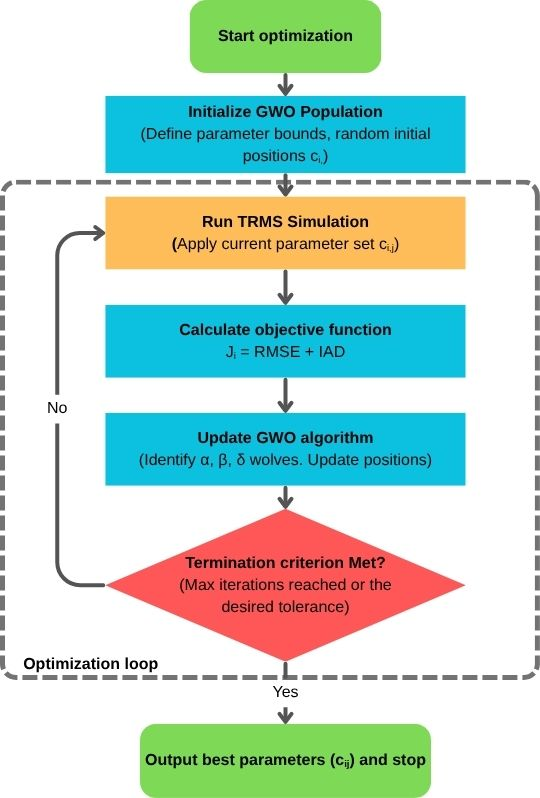
\includegraphics[width=8cm]{figure3/GWO_org.jpg} 
    \caption{Flowchart of the GWO optimization process for controller tuning.}
    \label{fig:gwo_optimization}
\end{figure}

To perform this optimization in a systematic and efficient manner, the Grey Wolf Optimizer (GWO) is employed, as extensively detailed in Chapter~\ref{chp2}. The GWO is a population-based metaheuristic algorithm inspired by the social hierarchy and cooperative hunting strategy of grey wolves. Its key advantage lies in its ability to simultaneously balance global exploration of the parameter space and local exploitation of promising regions, thereby avoiding premature convergence to suboptimal solutions. The optimization procedure adopted in this work is illustrated in Fig.~\ref{fig:gwo_optimization}. At each iteration, the population of candidate parameter sets is evaluated and ranked, and the positions of all wolves are updated according to the guidance of the three best solutions found so far (the alpha, beta, and delta wolves), progressively narrowing the search toward the optimal region.

To guide this search, an objective function $J$ is formulated to minimize the trajectory tracking error while simultaneously penalizing excessive or high-frequency variations in the control input. Specifically, considering the tracking error $e_{i,1}(k)$ and the control input $u_i(t)$ for each subsystem $i \in \{P, Y\}$, the composite objective function is defined as:
\begin{equation}
    J = \sum_{i \in \{P, Y\}} \left( \sqrt{\frac{1}{N} \sum_{k=1}^{N} e_{i,1}^2(k)} + \lambda_i \int_{0}^{T_{\text{sim}}} \left| \frac{du_i(t)}{dt} \right| dt \right)
    \label{eq:global_cost_function}
\end{equation}
The first term is the Root Mean Square Error (RMSE) between the desired and actual trajectories over $N$ discrete samples, which penalizes tracking inaccuracy. The second term is the Integral of the Absolute Derivative (IAD) of the control input over the simulation duration $T_{\text{sim}}$, which penalizes aggressive actuation and promotes signal smoothness. The weighting factor $\lambda_i$ balances the trade-off between these two competing objectives. This composite formulation ensures that the optimized controller not only achieves precise trajectory tracking but also generates smooth control inputs that are compatible with the physical limitations of the TRMS actuators. Since the vertical and horizontal subsystems share the same structure, a single global objective function $J = (J_v + J_h)/2$ is minimized over the entire system. The search behavior of the GWO is governed by two key parameters: the coefficient $a$, which decreases linearly from $2$ to $0$ over the course of iterations, gradually shifting the algorithm from broad exploration toward fine-grained exploitation of promising regions, and the random vectors $\vec{r}_1$ and $\vec{r}_2$, which are independently drawn from a uniform distribution in $[0, 1]$ at each iteration to introduce stochastic variability in the position update of each wolf. The optimized values of the gains $c_{i,1}$, $c_{i,2}$, and $c_{i,3}$ obtained through this process, along with the remaining controller parameters, are reported in the simulation section.

\section{Simulation Results and Discussion}
\label{sec:trms_results}

To evaluate the effectiveness and robustness of the proposed control strategy, a series of simulations were performed using the TRMS model within the MATLAB/Simulink environment. The initial conditions for all simulations were set to zero, defined as:
\begin{equation}
    \begin{cases}
        \mathbf{y}_{P}(0) = [y_{P,1}(0), y_{P,2}(0), y_{P,3}(0)]^T = [0,0,0]^T \\
        \mathbf{y}_{Y}(0) = [y_{Y,1}(0), y_{Y,2}(0), y_{Y,3}(0)]^T = [0,0,0]^T
    \end{cases}
\end{equation}
The remaining controller parameters were fixed as follows: $p = 107/100$, $a_{1,i} = a_{2,i} = 0.1$, $\gamma_{1,i} = 1$, $\beta_{1,i} = 1$, and $\gamma_{2,i} = \gamma_{3,i} = 4/3$. The two RBFNN estimators $\mathcal{W}_{1,i}^{T}\Phi_{1,i}$ and $\mathcal{W}_{2,i}^{T}\Phi_{2,i}$ each employ six nodes arranged in a standard three-layer architecture consisting of an input layer, a hidden layer, and an output layer. Each neuron in the hidden layer utilizes a Gaussian activation function with a width set to four. The centers of the Gaussian functions for the first and second estimators are defined as:
\begin{equation}
    \mu_{1,i} =
    \begin{bmatrix}
        -2 & -1 & 0 & 1 & 2 \\
        -2 & -1 & 0 & 1 & 2 \\
        -2 & -1 & 0 & 1 & 2 \\
        -2 & -1 & 0 & 1 & 2 \\
        -3 & -1 & 0 & 1 & 3 \\
        -3 & -1 & 0 & 1 & 3
    \end{bmatrix}, \quad
    \mu_{2,i} =
    \begin{bmatrix}
        -3 & -2 & -1 & 0 & 0 & 1 & 2 & 3 \\
        -3 & -2 & -1 & 0 & 0 & 1 & 2 & 3 \\
        -3 & -2 & -1 & 0 & 0 & 1 & 2 & 3 \\
        -3 & -2 & -1 & 0 & 0 & 1 & 2 & 3 \\
        -2 & -2 & -1 & 0 & 0 & 1 & 2 & 3 \\
        -2 & -2 & -1 & 0 & 0 & 1 & 2 & 3
    \end{bmatrix}
\end{equation}
The backstepping gains $c_{i,1}$, $c_{i,2}$, and $c_{i,3}$, which have the most direct and significant influence on both the tracking performance and the smoothness of the generated control signals, were optimized offline via the GWO algorithm. The optimized values are listed in Table~\ref{tab:control_parameters}. The simulations encompass various scenarios, including tracking of different reference signals, operation under external disturbances, and the presence of several types of sensor faults affecting the angular velocity measurements. These scenarios are designed to thoroughly test the Fixed-Time Adaptive Neural Controller (FxTANC) and its fault-tolerant version, the Fault-Tolerant Fixed-Time Adaptive Neural Controller (FTFxTANC).

\begin{table}[htbp]
\centering
\caption{Optimal control design parameters obtained via GWO.}
\label{tab:control_parameters}
\begin{tabular}{@{}llc@{}}
\toprule
\textbf{Parameter} & \textbf{Description} & \textbf{Value} \\ \midrule
$c_{P,1},\ c_{P,2},\ c_{P,3}$ & Pitch subsystem gains & $13.96,\ 47.30,\ 15.52$ \\ \midrule
$c_{Y,1},\ c_{Y,2},\ c_{Y,3}$ & Yaw subsystem gains   & $21.06,\ 50.00,\ 29.55$ \\
\bottomrule
\end{tabular}
\end{table}

\begin{figure}
    \centering
    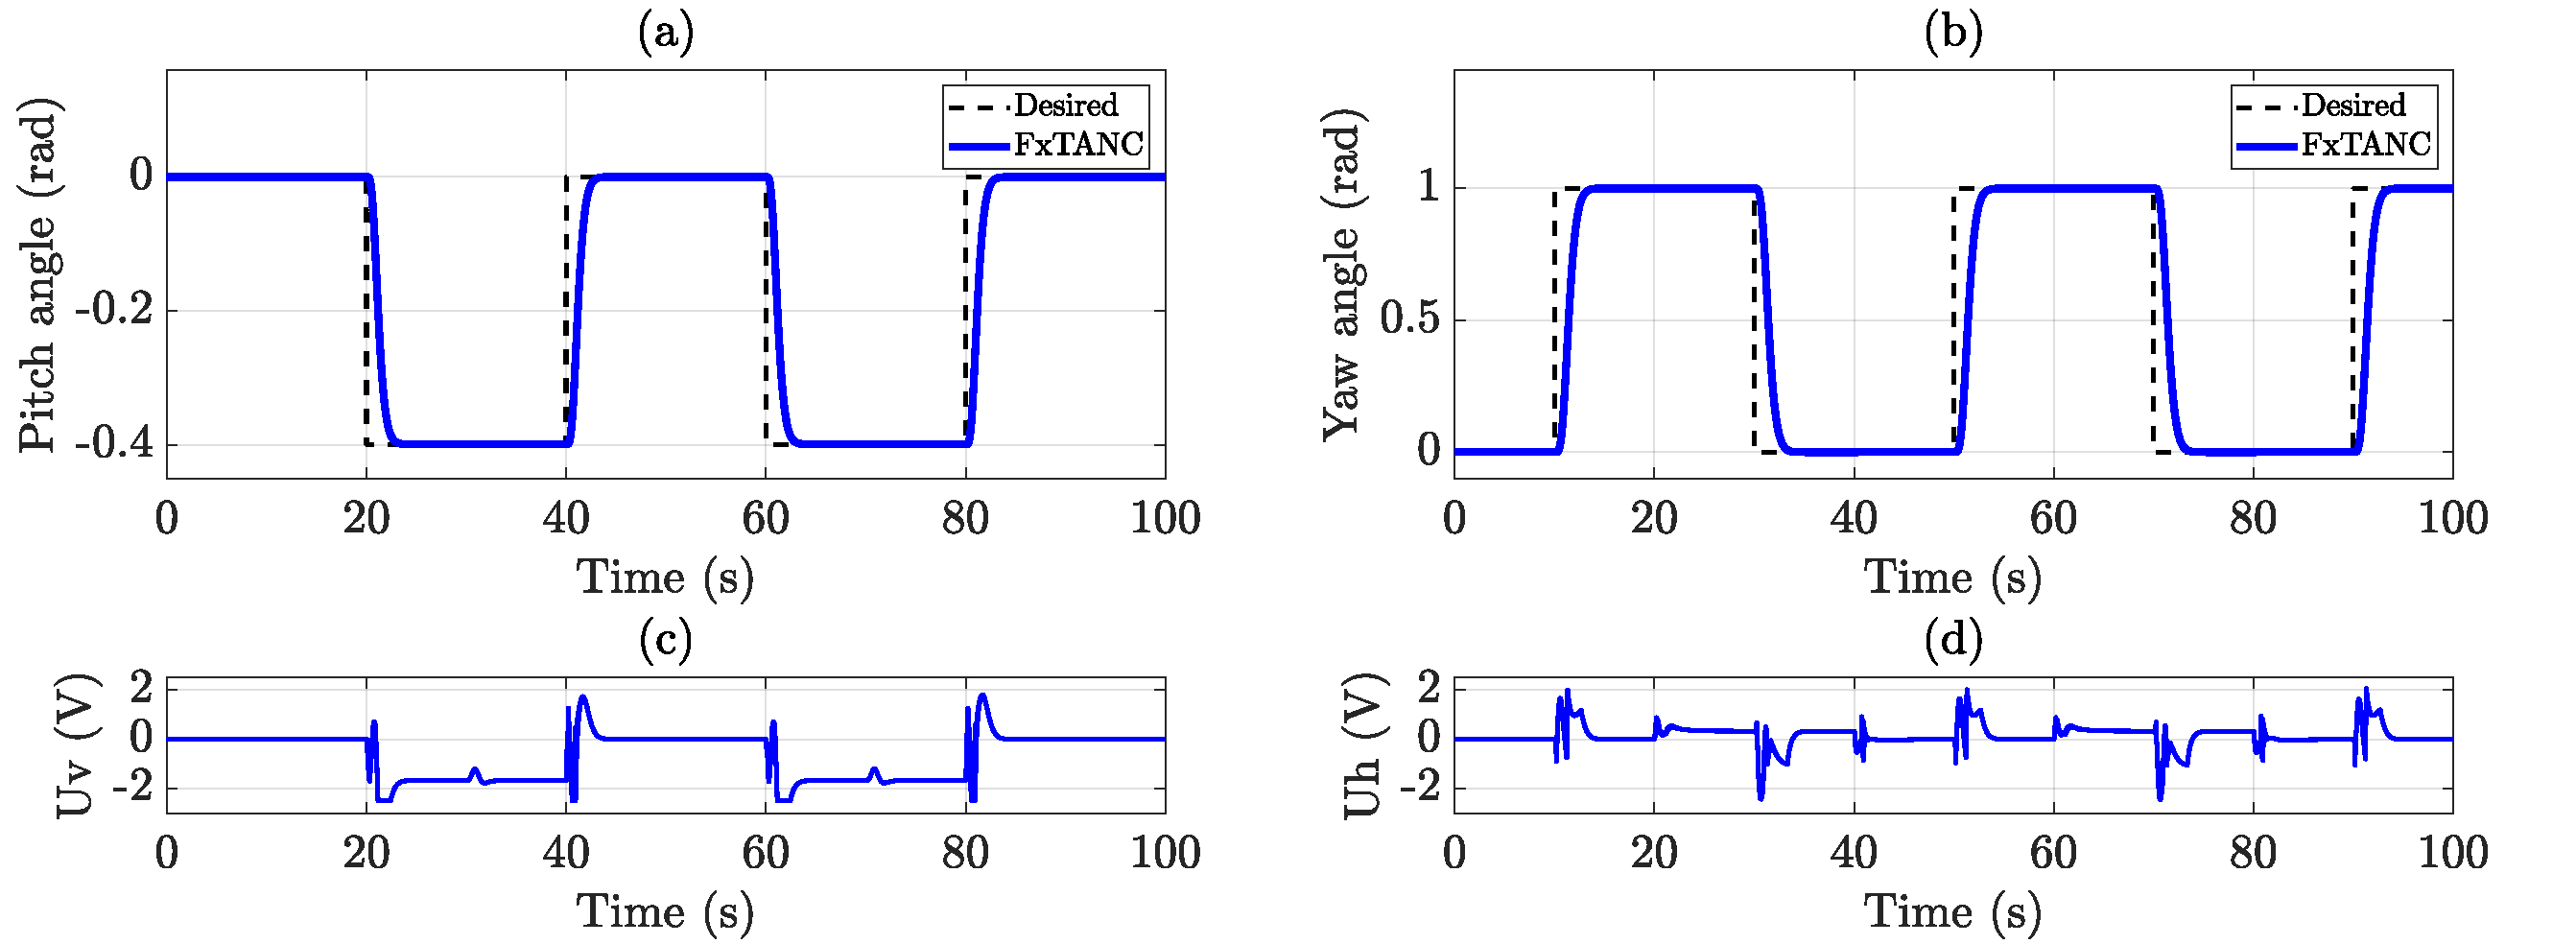
\includegraphics[width=14cm]{figure3/square.pdf}
    \caption{TRMS response to square-wave references showing attitude tracking and corresponding control inputs. \label{sqr}}
\end{figure}

\subsection{Case 1: Square-Wave Reference Tracking}
The initial evaluation focused on the system's ability to track square-wave reference signals for both pitch and yaw angles using the FxTANC, without the introduction of faults or the fault estimation mechanism. As depicted in Fig.~\ref{sqr}, the pitch ($\alpha_P$) and yaw ($\alpha_Y$) angles successfully follow their respective desired square-wave trajectories. This demonstrates the controller's capability to manage the inherent cross-coupling between the vertical (pitch) and horizontal (yaw) dynamics of the TRMS, even with abrupt changes in the reference signals. Furthermore, the corresponding control input voltages, $v_P$ and $v_Y$, shown in Fig.~\ref{sqr} (c,d), remain well within the predefined operational limits of $\pm 2.5V$, which is essential for practical implementation and actuator integrity. This scenario confirms the baseline performance and stability of the FxTANC under ideal conditions.

\begin{figure}
    \centering
    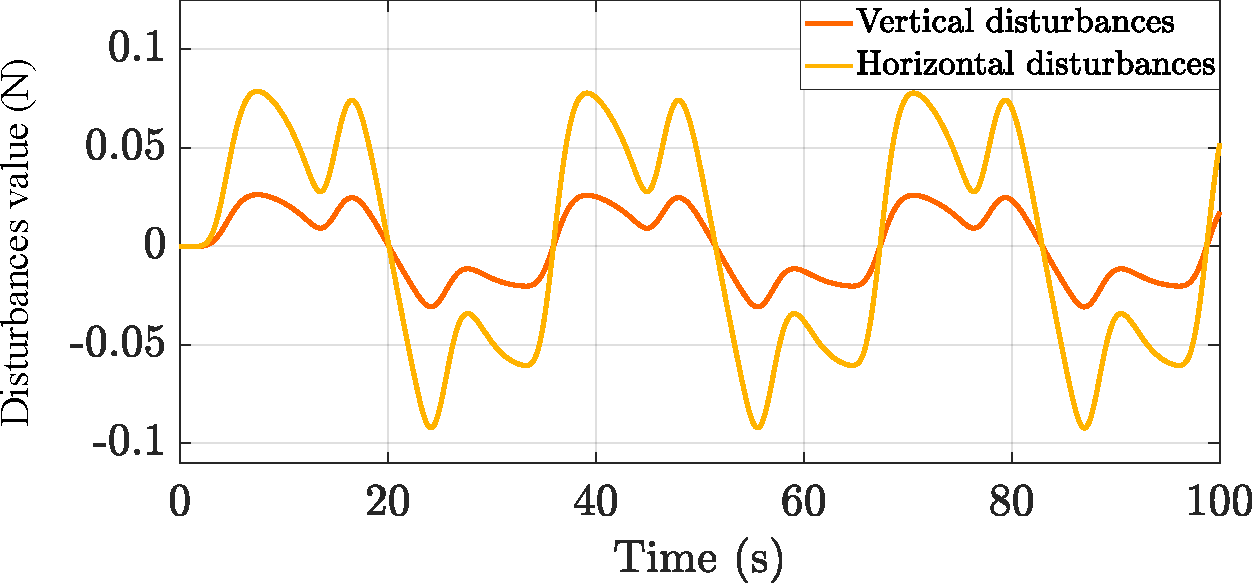
\includegraphics[width=7cm]{figure3/d.pdf}
    \caption{External disturbance profiles applied to the vertical and horizontal dynamics of the TRMS. \label{dis}}
\end{figure}

\begin{figure}
    \centering
    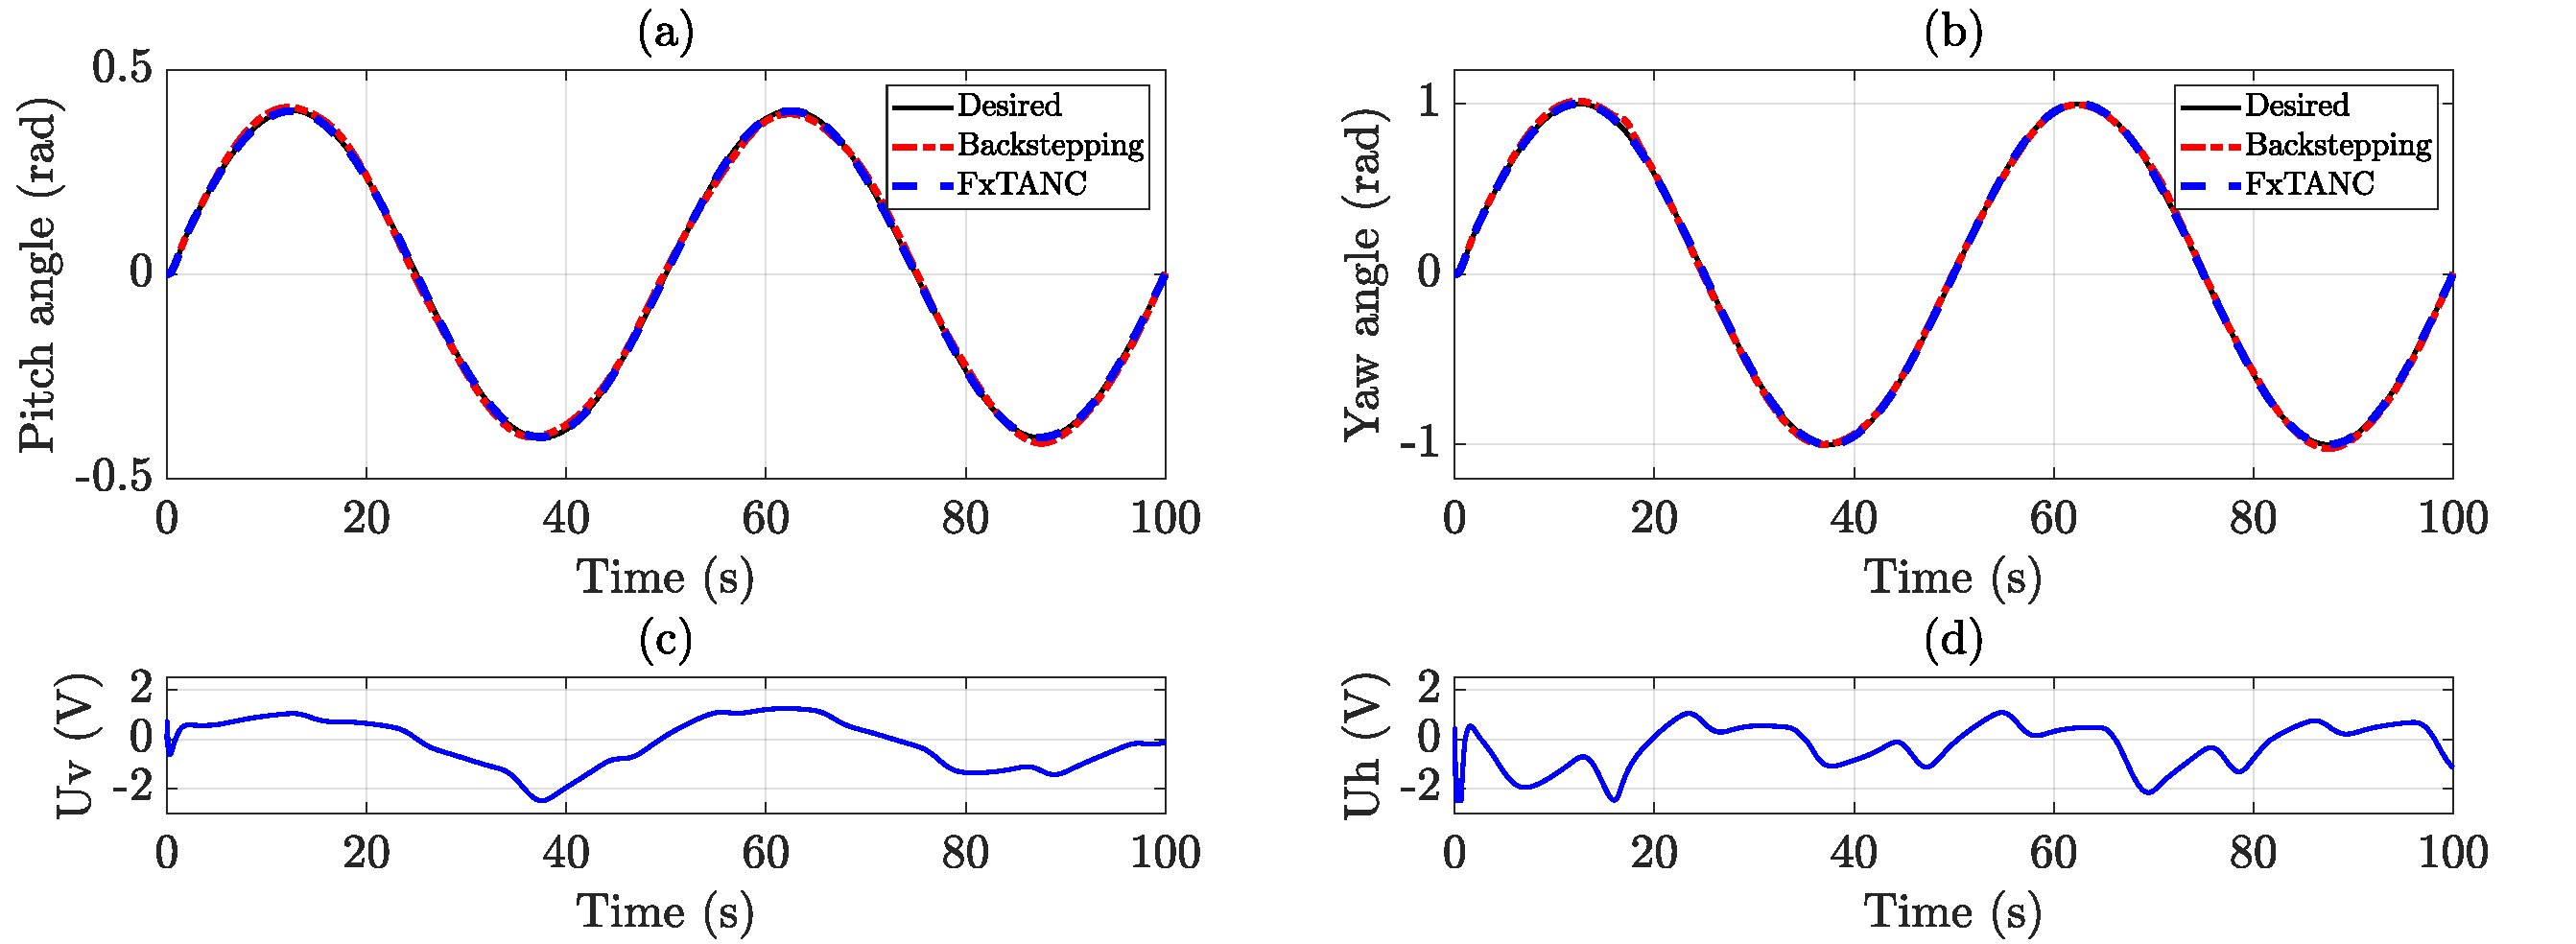
\includegraphics[width=14cm]{figure3/sine.pdf}
    \caption{Attitude and control input response of the TRMS under sinusoidal tracking with external disturbances. \label{faultfree}}
\end{figure}

\subsection{Case 2: Sinusoidal Reference Tracking with External Disturbances}
In the second scenario, the FxTANC was challenged with tracking sinusoidal reference signals, defined as $y_{d,P}(t) = 0.4\sin(0.02t)$ for pitch and $y_{d,Y}(t) = \sin(0.02t)$ for yaw, while subjected to external disturbances. The profiles of these disturbances, affecting both vertical and horizontal dynamics, are illustrated in Fig.~\ref{dis}. The system's response, presented in Fig.~\ref{faultfree}, showcases the robustness of the proposed FxTANC. When compared with a nominal backstepping controller (as referenced in the source paper), the FxTANC demonstrates superior tracking accuracy for both pitch and yaw angles (Fig.~\ref{faultfree} (a,b)), maintaining close adherence to the desired trajectories despite the persistent disturbances. The control input voltages for the main and tail rotors, shown in Fig.~\ref{faultfree} (c,d), are observed to operate within acceptable and constrained ranges, underscoring the controller's efficiency.

\begin{figure}
    \centering
    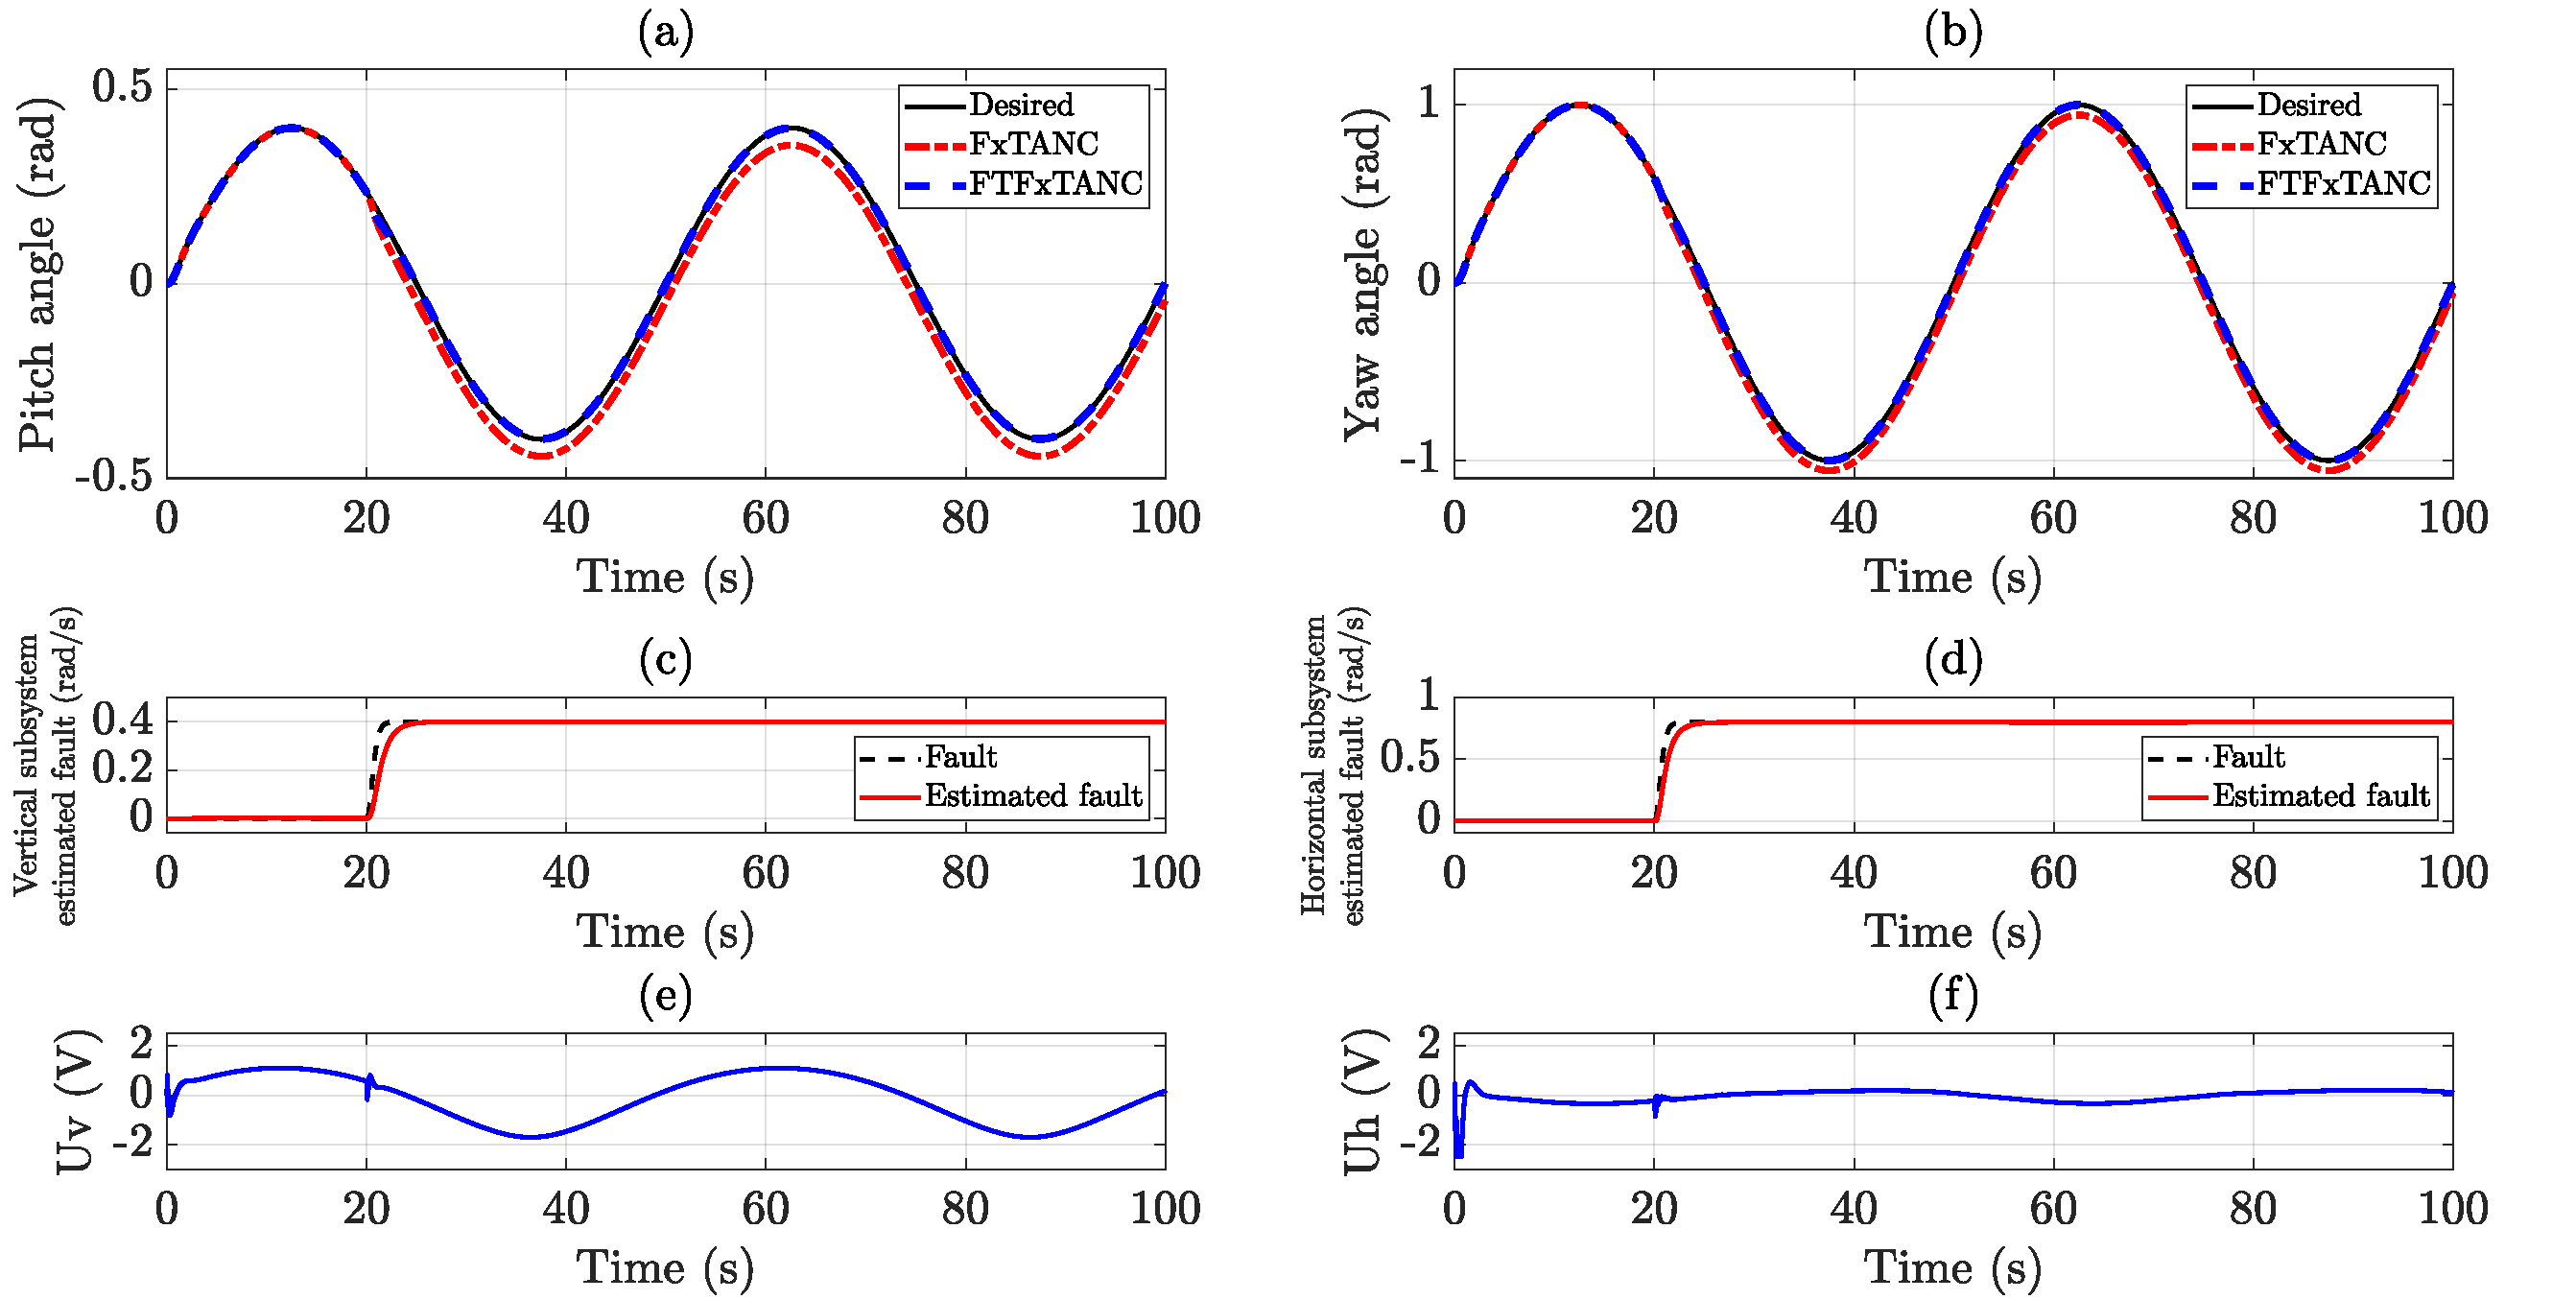
\includegraphics[width=14cm]{figure3/bias.pdf}
    \caption{System performance and fault estimation under sensor bias faults during sinusoidal tracking. \label{bias}}
\end{figure}

\subsection{Case 3: Performance under Sensor Bias Faults}
This test evaluates the performance of the FTFxTANC when confronted with bias faults in the angular velocity sensors. A bias fault was introduced at $t_f = 20s$, with magnitudes of $g_{A,P}(t) = 0.4 \, \text{rad/s}$ for the pitch sensor and $g_{A,Y}(t) = 0.8 \, \text{rad/s}$ for the yaw sensor. The simulation results are displayed in Fig.~\ref{bias}. The attitude tracking performance (Fig.~\ref{bias} (a,b)) demonstrates that the FTFxTANC effectively mitigates the impact of these bias faults, ensuring stable and accurate tracking of the sinusoidal references. In contrast, the FxTANC (without the fault-tolerant mechanism) would exhibit degraded performance. The adaptive fault estimation mechanism, whose outputs are shown in Fig.~\ref{bias} (c,d), successfully identifies and compensates for the introduced sensor biases. The control input voltages, depicted in Fig.~\ref{bias} (e,f), remain within appropriate bounds, highlighting the controller's ability to adapt to the faulty sensor readings without demanding excessive control effort.

\begin{figure}
    \centering
    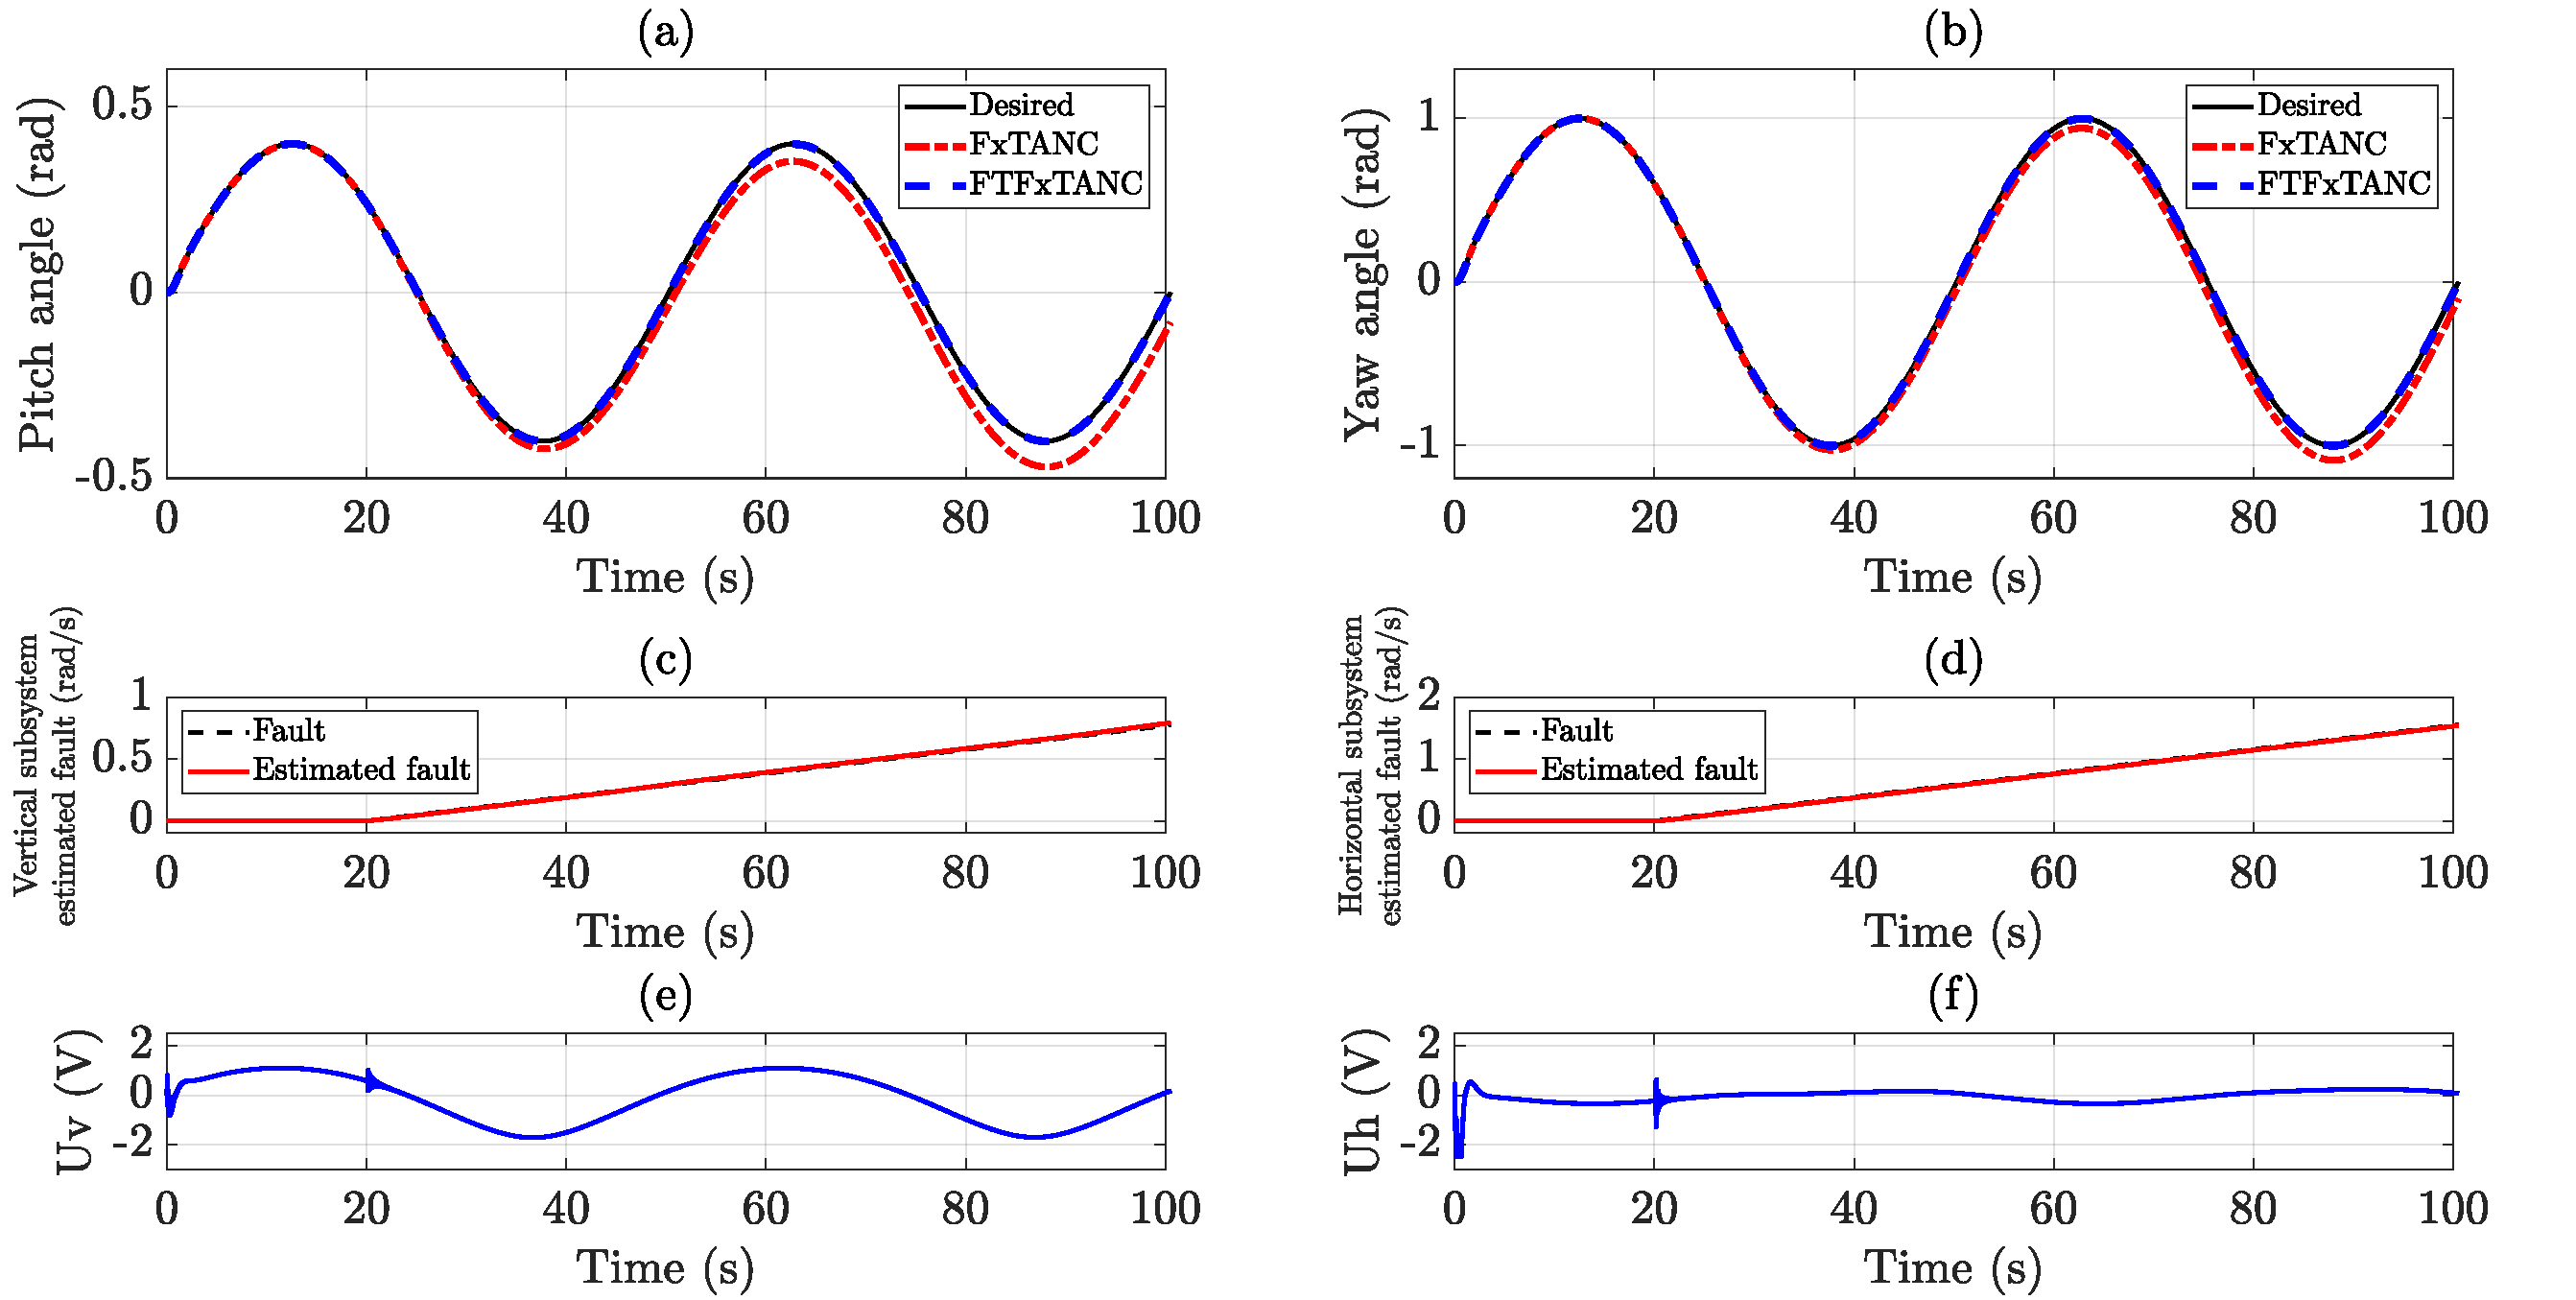
\includegraphics[width=14cm]{figure3/drift.pdf}
    \caption{TRMS attitude response, fault estimation, and control signals under sensor drift fault conditions. \label{drift}}
\end{figure}

\subsection{Case 4: Performance under Sensor Drift Faults}
The robustness of the FTFxTANC was further assessed against sensor drift faults affecting the angular velocity measurements. These faults were introduced at $t_f = 20s$ with drift coefficients of $g_{A,P}(t) = 0.01t$ for pitch and $g_{A,Y}(t) = 0.02t$ for yaw, simulating a scenario where small deviations accumulate over time. Fig.~\ref{drift} presents the system's response to this type of fault. The attitude tracking plots (Fig.~\ref{drift} (a,b)) indicate that the FTFxTANC effectively handles the drift fault, maintaining the TRMS on its desired trajectory despite the progressively deteriorating sensor information. The performance of the adaptive fault estimator is shown in Fig.~\ref{drift} (c,d), illustrating its capability to track and compensate for the time-varying drift. The control signals, depicted in Fig.~\ref{drift} (e,f), remain within safe operational limits, demonstrating the controller's adaptive capabilities in managing such faults.

\begin{figure}
    \centering
    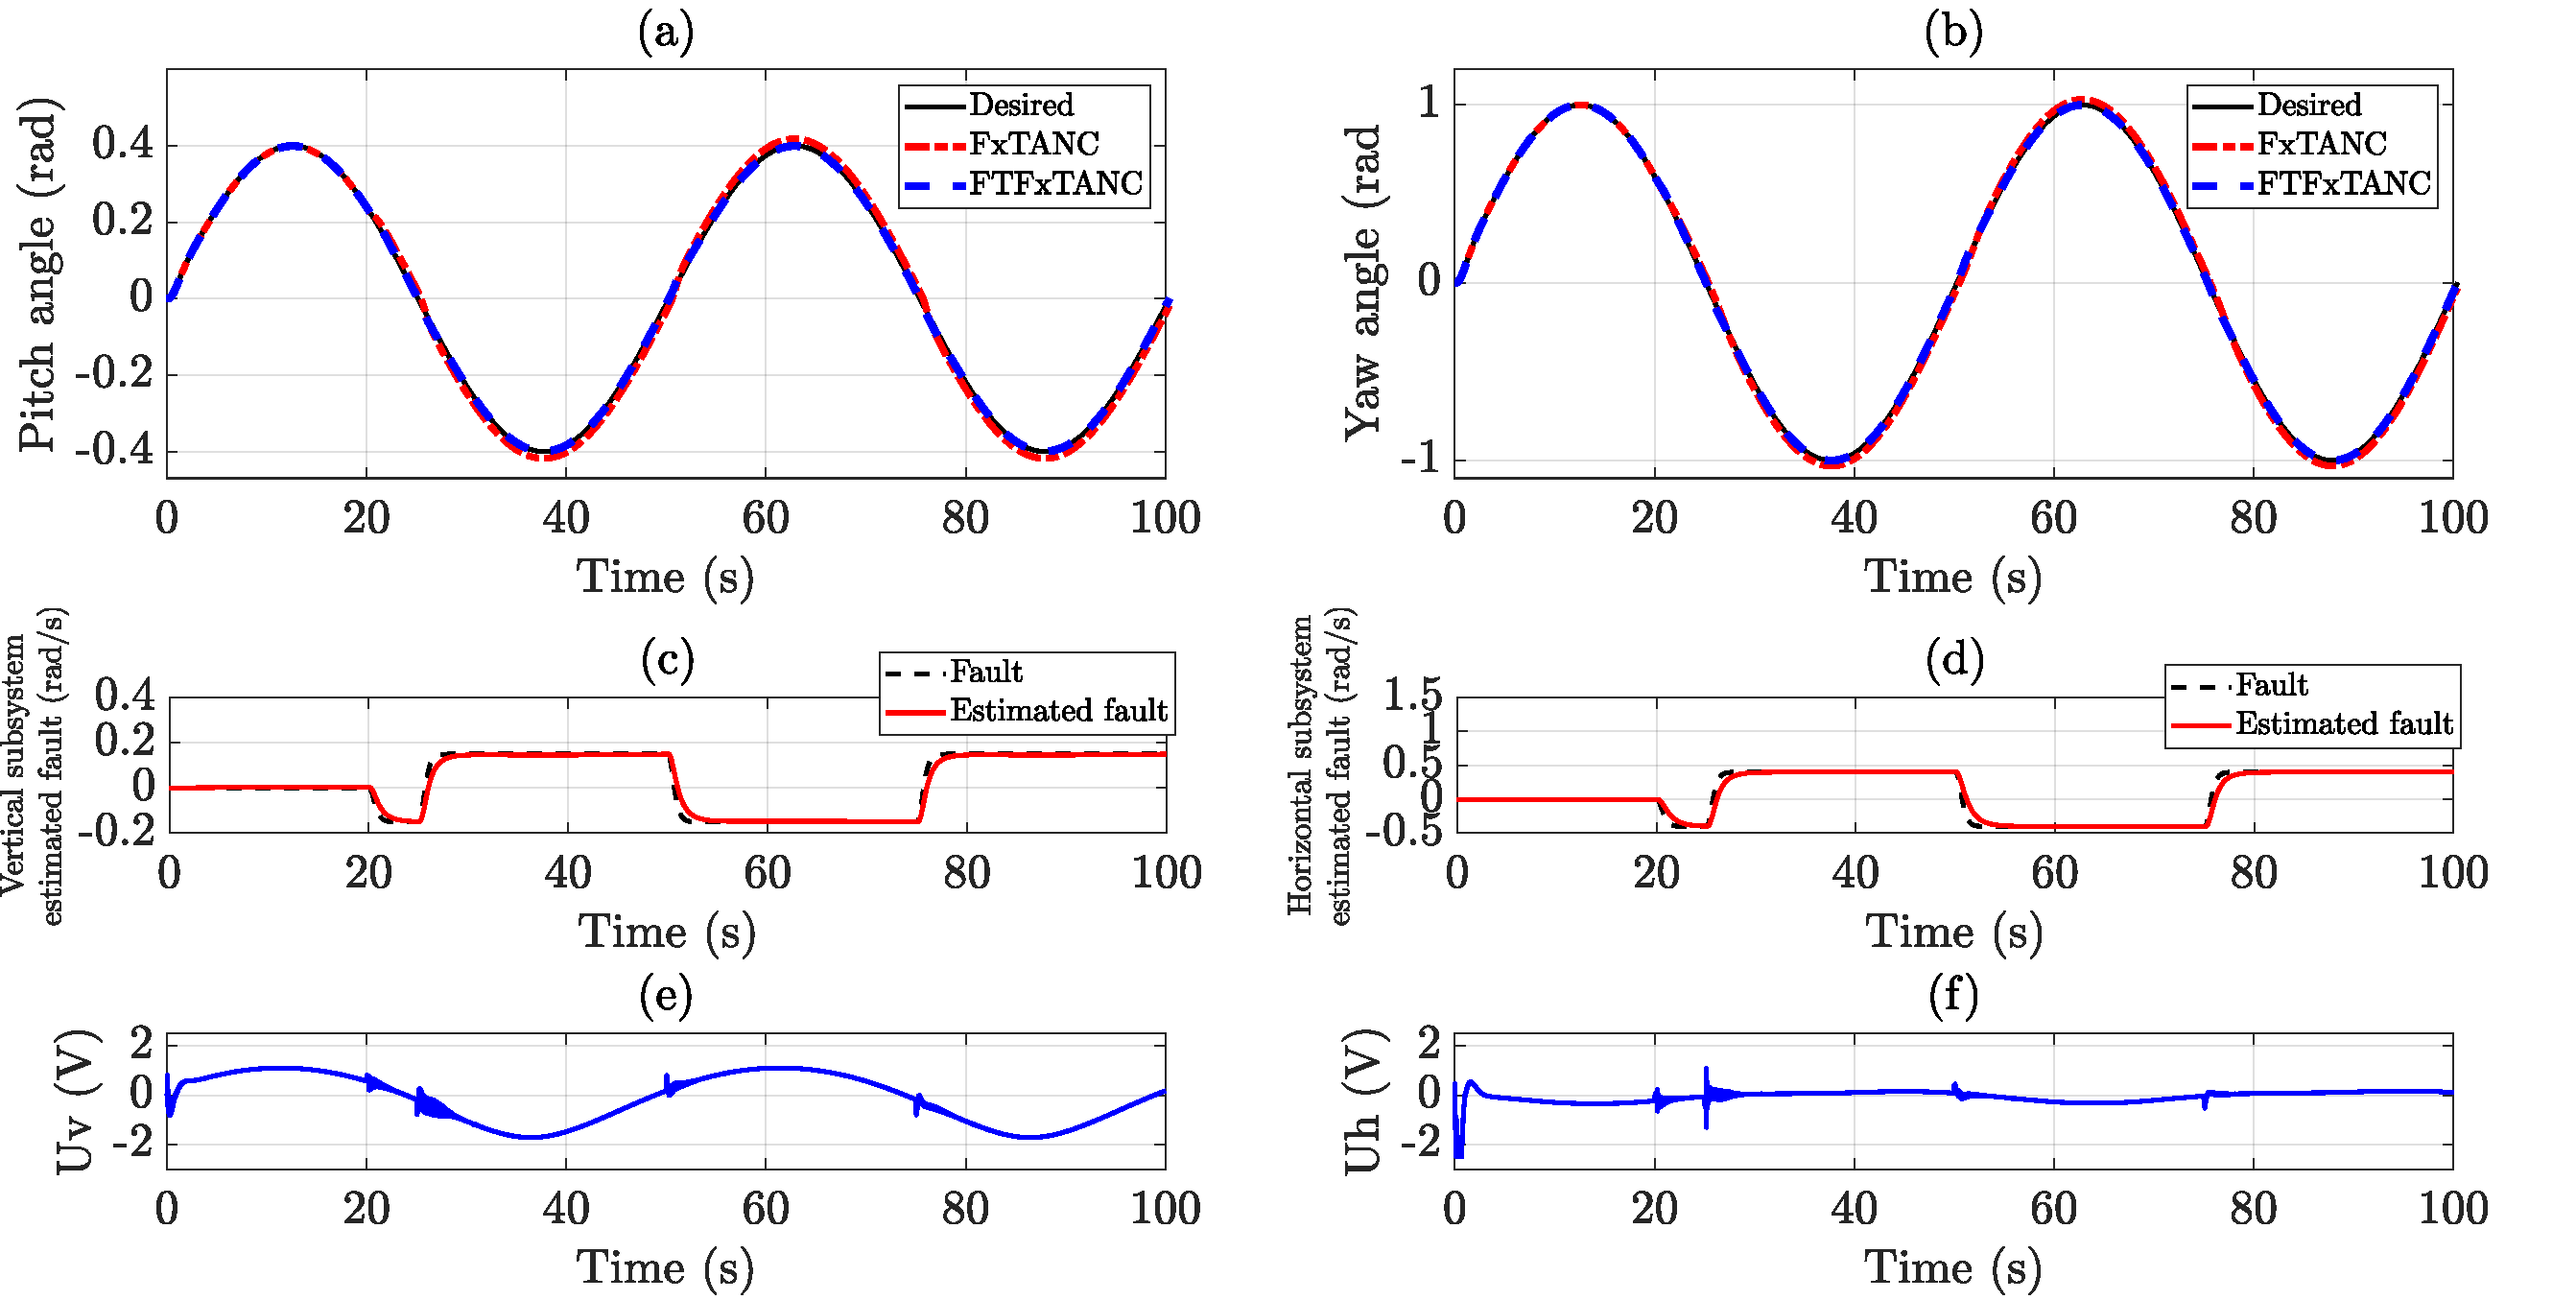
\includegraphics[width=14cm]{figure3/loa.pdf}
    \caption{TRMS attitude response, fault estimation, and control signals under loss of accuracy fault conditions. \label{lossOfAccuracy}}
\end{figure}

\subsection{Case 5: Performance under Loss of Accuracy in Sensors}
This scenario investigates the controller's performance when the TRMS velocity sensors experience a loss of accuracy, leading to incorrect and noisy readings. This fault condition was simulated by introducing an additive random noise fault at $t_f = 20s$, with maximum amplitudes of $|g_{A,P}(t)| = 0.15 \, \text{rad/s}$ (for pitch) and $g_{A,Y}(t) = 0.4 \, \text{rad/s}$ (for yaw). The results are shown in Fig.~\ref{lossOfAccuracy}. The pitch and yaw angle responses (Fig.~\ref{lossOfAccuracy} (a,b)) confirm that the proposed FTFxTANC can effectively manage this type of sensor degradation, maintaining satisfactory tracking performance. The fault estimation plots (Fig.~\ref{lossOfAccuracy} (c,d)) illustrate how the estimator identifies and counteracts the effects of the accuracy loss. Correspondingly, the control input voltages (Fig.~\ref{lossOfAccuracy} (e,f)) are shown to remain within acceptable ranges, affirming the controller's robustness.

\begin{figure}
    \centering
    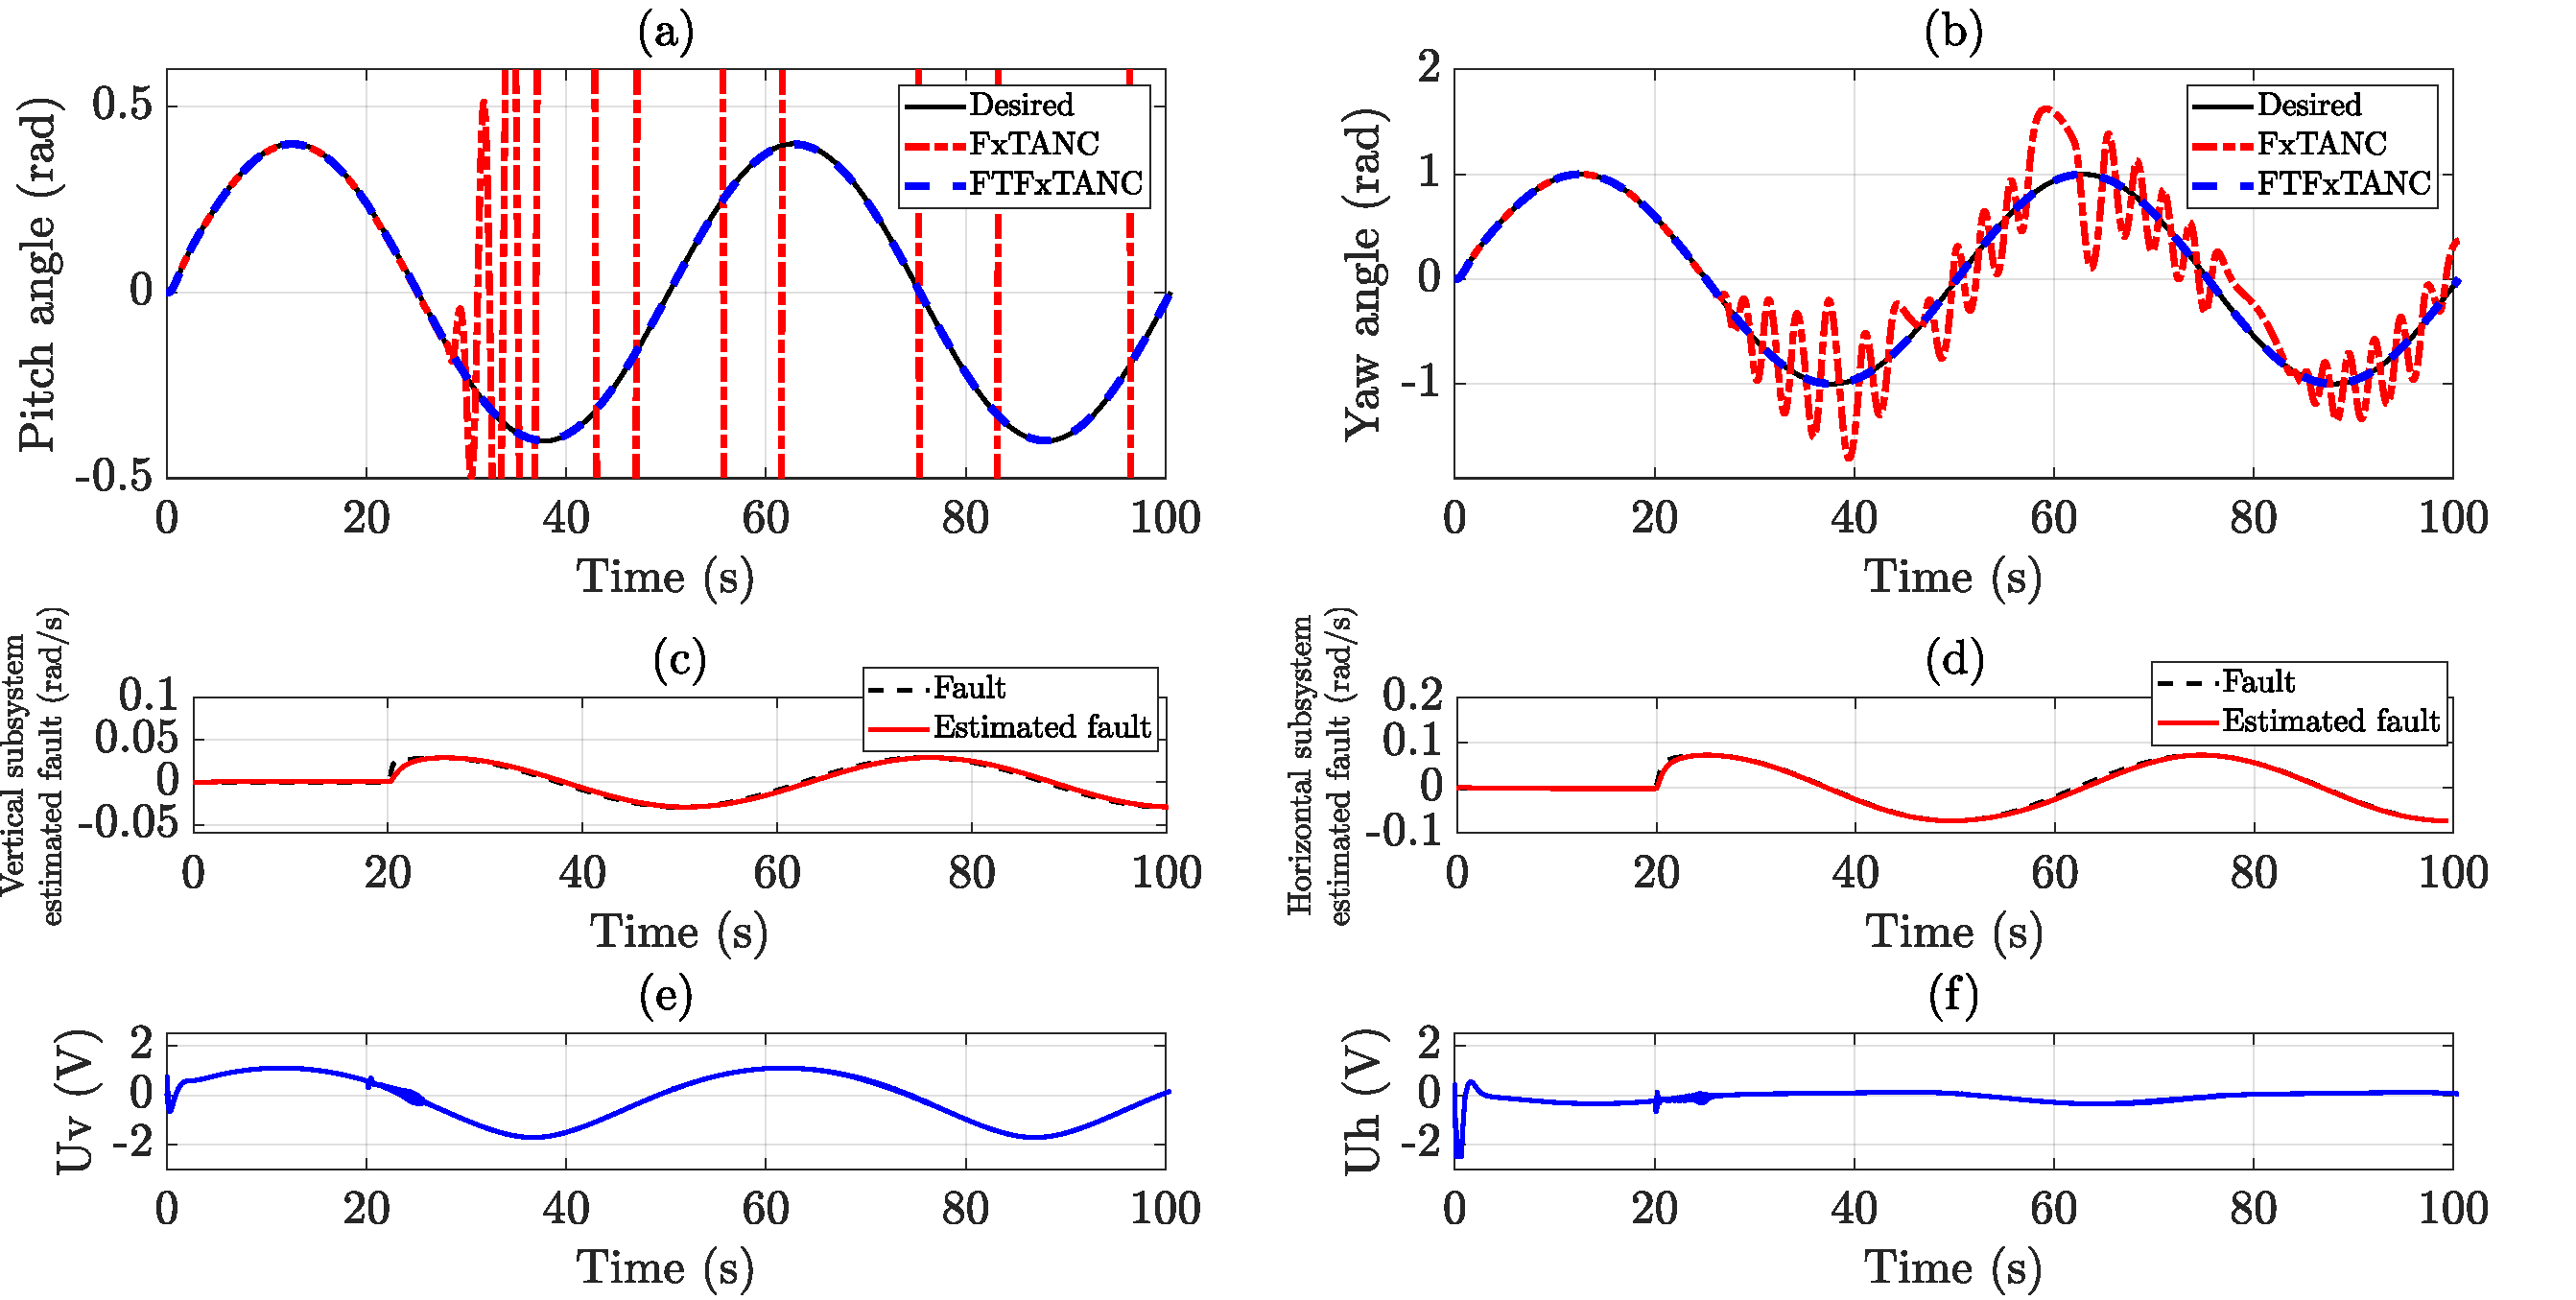
\includegraphics[width=14cm]{figure3/loe.pdf}
    \caption{TRMS attitude response, fault estimation, and control signals under sensor loss of effectiveness fault conditions. \label{lossOfEffectiveness}}
\end{figure}

\subsection{Case 6: Performance under Loss of Effectiveness in Sensors}
The final simulation case examines the FTFxTANC's ability to handle a loss of effectiveness in the angular velocity sensors. This fault type implies that the sensor readings are scaled down, providing only a percentage of the true value. A 55\% reduction in sensor effectiveness was introduced at $t_f = 20s$. The system's response is detailed in Fig.~\ref{lossOfEffectiveness}. The attitude tracking performance (Fig.~\ref{lossOfEffectiveness} (a,b)) clearly shows that the FTFxTANC successfully manages this significant sensor fault, maintaining close adherence to the desired trajectories. In contrast, the FxTANC (without fault tolerance) is shown to become unstable and exhibit degraded performance under such a fault. The fault estimation subsystem (Fig.~\ref{lossOfEffectiveness} (c,d)) accurately detects and compensates for this multiplicative fault, demonstrating the robustness of the integrated fault-tolerant design. The control voltages generated by the FTFxTANC (Fig.~\ref{lossOfEffectiveness} (e,f)) remain stable and within permissible operational limits, further validating the controller's effectiveness.

\subsection{Summary of Results}
The collective simulation results presented across these varied scenarios demonstrate the capabilities of the proposed control strategy. The FxTANC shows excellent tracking performance under nominal conditions and in the presence of external disturbances. More significantly, the FTFxTANC exhibits remarkable resilience and fault tolerance when faced with diverse sensor fault types, including bias, drift, loss of accuracy, and loss of effectiveness. In all tested fault scenarios, the FTFxTANC maintained stable operation and accurate trajectory tracking, while the adaptive fault estimators effectively identified and compensated for the sensor failure. The control inputs consistently remained within practical limits, highlighting the controller's efficiency and suitability for real-world TRMS applications. These findings underscore the effectiveness of combining fixed-time stability concepts with adaptive neural networks and dedicated fault estimation mechanisms for complex UAV systems.

\section{Summary}
\label{sec:trms_conclusion}
This chapter presented a fixed-time fault-tolerant control strategy for a twin-rotor UAV system using adaptive neural networks. The selected platform (TRMS) was chosen for its helicopter-like configuration and dynamic complexity, making it an ideal benchmark for evaluating advanced control techniques. The primary objective was to ensure robust trajectory tracking performance despite unknown nonlinear dynamics, external disturbances, and sensor faults.

To achieve this goal, the proposed control scheme was developed based on the backstepping technique integrated with NNs for approximating unknown system behaviors. A decentralized structure was adopted to simplify the control of pitch and yaw dynamics of the TRMS, each one treated independently. The controller also actively estimated and compensated for sensor faults such as bias, drift, accuracy loss, and loss of effectiveness through an adaptive estimation mechanism.

A key innovation of this chapter was the incorporation of fixed-time stability, which ensures system convergence within a predefined time frame regardless of initial conditions. This is a significant advantage for safety-critical aerial missions. Furthermore, the GWO algorithm was employed to automatically tune the control gains, enhancing system performance without requiring manual parameter tuning.\\
Simulation results validated the effectiveness and robustness of the proposed approach under various scenarios, including normal operation, external disturbances, and different types of sensor faults. Compared to traditional methods, the proposed controller demonstrated superior fault resilience, faster convergence, and bounded control effort.\\
In summary, the developed control framework offers a powerful, adaptive, and fault-resilient solution for twin-rotor UAVs, and it sets a strong foundation for extending similar methodologies to more complex aerial vehicles in the subsequent chapters.

